% Is Wireless Encryption Ready for the AI Era?
% Anonymized submission manuscript (double-blind). No author information.
% Compile from the submission/ directory: pdflatex manuscript.tex (twice).
\documentclass[11pt,a4paper]{article}
\usepackage{booktabs}
\usepackage{array}
\usepackage{tabularx}
\usepackage{graphicx}
\usepackage[top=1in,bottom=1in,left=1in,right=1in]{geometry}
\usepackage[colorlinks=true,linkcolor=blue,urlcolor=cyan,citecolor=blue]{hyperref}
\usepackage{url}

\title{Is Wireless Security Ready for the AI Era?\\A Structured Scoping Review and Classification of 130 Studies, 2020--2026}
\author{Anonymous Authors\\{\small Anonymized for double-blind review}}
\date{}

\begin{document}
\sloppy
\maketitle

\begin{abstract}
Machine learning (ML) is now central to published radio-link authentication research---and simultaneously the adversary's standard toolkit. This structured scoping review classifies a 121-study core (2020--2026) on ML for wireless-link security or attacks on it---84 defense, 30 threat, and 7 dual attack-plus-defense studies---plus 9 post-quantum contextual studies kept separate (130 total). Each paper is coded by function, method family, data source, validation, and readiness. Scope: authentication/RFFI, key generation, anti-jamming, classifier-as-boundary analysis, federated privacy. The title answer is no for the research literature: defenses optimize accuracy while threats demonstrate exploits, and readiness evidence trails accuracy claims.

Deep supervised learning leads (45) over adversarial ML (40, peaking at 11 in 2024); reinforcement learning holds at 9 defense-side papers, with a single LLM-assisted fuzzer (2026). Authentication/RFFI absorbs 69 of 121 core (57.0\%); anti-jamming (14), key generation (12), federated privacy (11), and protocol/traffic analysis (10) follow.

Three weaknesses persist. First, validation is split by kind: 16 of 30 threat studies demonstrate on testbeds, and closed-loop evaluation is found in at least 14 of 121 core (11.6\%; dual-track realism figures in \S\ref{sec:cross}, not here). Second, reproducibility is near-absent (4 verified artifact releases among 121 core, 3.3\%, a lower bound) and standards alignment weakest outside the PQC stratum (12 of 121 core rows carry any standards signal, 9.9\%---6 defense and 1 dual R5>0 plus 5 attack rows naming an affected standard). Third, real-time, update, and multi-agent-trust needs are essentially unaddressed (1--2 papers each). Validation rigor runs close across channels with gaps small relative to arm sizes; channel timing is assessed in \S\ref{sec:sensitivity}. A twelve-item reporting checklist closes the paper.
\end{abstract}

\noindent\textbf{Keywords:} wireless security; physical-layer authentication; RF fingerprinting; adversarial machine learning; physical-layer key generation; anti-jamming; post-quantum migration; scoping review.

\section{Introduction}
\label{sec:intro}
\subsection{The radio link under AI pressure}
Wireless links broadcast by physics: every transmission is receivable by anyone in range, which makes the radio link the natural attack surface for interception, impersonation, and jamming. The classical answer---encryption, authentication and key agreement (AKA), and physical-layer techniques---now faces three simultaneous strains. First, software-defined radios put laboratory-grade interception and transmission in every adversary's hands. Second, machine learning turns raw captures into fingerprints, keys, and exploits automatically, without hand-built demodulators. Third, autonomous systems (drones, vehicles, swarms, IoT/edge fleets) need authentication under real-time deadlines, over-the-air updates, and multi-agent trust---requirements the literature rarely addresses together. The question this review asks is whether the radio-link security literature has kept pace with the adversary it has itself equipped.

\subsection{How AI entered wireless security}
AI entered through authentication. Deep networks learned RF fingerprints from raw I/Q, outperforming hand-crafted features, and physical-layer key generation promised lightweight secrets from channel reciprocity without public-key infrastructure. The adversarial turn followed quickly: white-box FGSM/PGD perturbations and black-box universal perturbations (81.7\% success with almost no victim knowledge) break RFFI classifiers on real LoRa captures [T03]; reinforcement-learned impersonation needs only binary accept/reject feedback for $>$90\% penetration [T18] (an adversarial-ML attack---the defense-side DRL family counts control methods only, so Fig.~\ref{fig:methodtrack} shows no DRL threat rows); GAN-spoofed signals pass PHY authentication at 76\% [T09]. Two results reset expectations for the field: far-field deep-learning side-channel recovery of BLE AES-128 at 15~m from fewer than 400 traces [T01], and Magmaw [T30] (NDSS'25)---protocol- and modality-agnostic universal perturbations, SDR-demonstrated at noise-level power, surviving adversarial training, subtraction, detection, and oracle defenses, including against an encrypted image channel. Authentication learned from waveforms, it turned out, could be unlearned by waveforms. Fig.~\ref{fig:milestones} places these turning points on a timeline: with two exceptions (a 2022 ensemble defense and a 2025 proactive-authentication defense), every milestone is an attack (milestones author-selected to mark field turns, not sampled).
\begin{figure}[tbp]
\centering
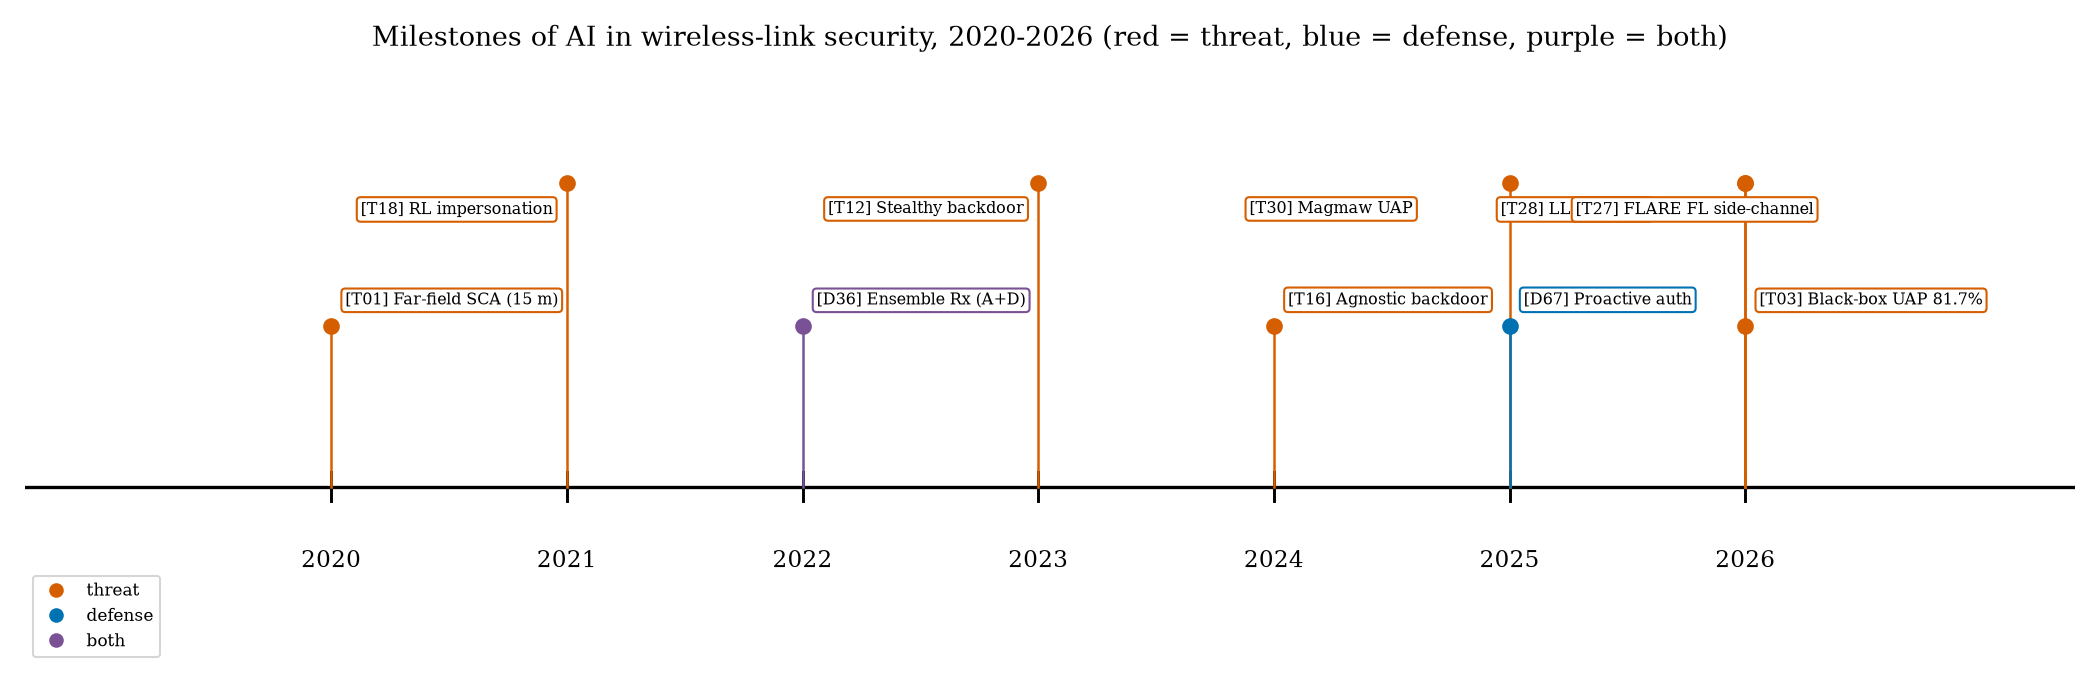
\includegraphics[width=\linewidth]{figures/FigC_milestones.png}
\caption{Milestones of AI in wireless-link security, 2020--2026. Red markers are threats, blue defenses, purple joint attack-plus-defense work.}
\label{fig:milestones}
\end{figure}

\subsection{Existing reviews and the literature gap}
The review literature has grown alongside the applications, but it is fragmented along the same axes as the primary studies. Function-specific surveys cover RF fingerprinting [BG3]; method-specific ones follow adversarial ML [BG7]; the closest cross-functional account is a physical-layer-authentication survey for the ML era [BG2]. Table~\ref{tab:priors} compares their scope and method against this review. What is largely missing is a cross-functional, quantitative account of the field's trajectory: which AI method families are actually being used for which security functions, on which data, validated how, and how that picture has shifted over 2020--2026. This gap matters because the field's self-image drives its research allocation. If most published authenticators are validated on closed-set, single-receiver, static-channel benchmarks, the community's sense of progress is calibrated to a regime that differs sharply from deployment under adaptive adversaries. Answering such questions requires a corpus-level, cross-functional account rather than another narrative synthesis of one function.

\begin{table}[tbp]
\centering
\footnotesize
\caption{Prior surveys closest to this review: scope, method, and what differs here.}
\label{tab:priors}
\begin{tabular}{@{}l p{3.6cm} p{2.6cm} p{5.2cm}@{}}
\toprule
Survey & Scope & Method & This review instead \\
\midrule
{[BG3]} Jagannath 2022 & RFFI only & Narrative & 8 functions quantified jointly \\
{[BG7]} Adesina 2023 & Adversarial wireless ML & Narrative & Plus defenses, validation grade, trends \\
{[BG2]} Hoang 2024 & PLA/auth in ML era & Narrative & Plus threats, readiness scores, checklist \\
\bottomrule
\end{tabular}
\end{table}

\subsection{Contribution of this paper}
This paper makes four contributions. First, it assembles a verified corpus of 121 core studies (2020--2026) on AI in wireless-link security broadly construed, plus 9 post-quantum contextual studies kept in a separate stratum (130 records total) (authentication, key generation, secure communications/anti-jamming, signal/traffic analysis where the classifier is the security boundary, federated privacy, plus a separate PQC-context stratum), in which every record carries a resolvable identifier verified record-by-record (journal/conference DOI, arXiv/ePrint ID, USENIX paper URL, or publisher landing page---no identifier fabricated, none shared: two initially mis-keyed records were corrected against publisher metadata (D20 to its TVT paper, D55 to its TCCN paper)). Two same-team companion pairs are counted as distinct records with disclosure (D55/T15: TCCN authorization framework plus datasets vs GLOBECOM outlier-augmentation method---the arXiv preprint carries the GLOBECOM title and cites the TCCN paper as prior work, confirming distinct records; D20/T20: TVT UAV-PLA paper vs CPS-IoT Week encrypted-traffic paper); dropping either pair would move N to 129/128 without changing headline patterns. One same-team conference-to-journal extension was deduped (T02 subsumed by T03, which covers its FGSM/PGD results and adds black-box UAP). Second, it develops a two-axis classification framework---security function $\times$ AI method family---extended with track, data-source, validation-practice, and readiness fields, and applies it uniformly to all 130 papers. Third, it quantifies the field's six-year evolution across functions, methods, data, and validation (\S\ref{sec:corpus}), identifying the shift from deep supervised fingerprinting through adversarial ML to DRL anti-jamming, federated privacy, and early LLM-assisted analysis. Fourth, it provides a critical, function-by-function review of what the corpus actually demonstrates (\S\S\ref{sec:threat}--\ref{sec:pqc}), a cross-cutting analysis of the threat--defense asymmetry (\S\ref{sec:cross}), and distills a gap-driven research agenda plus a reporting checklist (\S\ref{sec:gaps}).
Fig.~\ref{fig:heatmap} previews the analysis, mapping the corpus across security functions and method families: the field's center of gravity sits squarely in the RFFI $\times$ (adversarial $+$ deep-supervised) complex, key generation is a simulation-heavy island, and LLM-assisted work is only now appearing. The remainder of the paper is organized as follows. \S\ref{sec:methods} details the review methodology. \S\ref{sec:corpus} presents the corpus overview and bibliometric analysis. \S\S\ref{sec:threat}--\ref{sec:pqc} review threats, defenses, and the quantum-era context. \S\ref{sec:cross} examines cross-cutting directions. \S\ref{sec:gaps} formulates gaps and the checklist. \S\ref{sec:conclusion} concludes.

\section{Review Methodology}
\label{sec:methods}
\subsection{Scope and objective}
The objective is to characterize the state and evolution of AI applied to radio-link security broadly construed: authentication/RFFI (including localization-fingerprint attacks where geofence bypass breaks an authorization boundary), key generation/distribution/exchange/management, anti-jamming/secure communications, protocol/traffic/signal analysis where the classifier is the security boundary, side-channel analysis, federated privacy, and learned primitives---crossed with AI as attacker tool, defender tool, or learned primitive---over 2020-01-01--2026-10-11, plus readiness gaps for autonomous systems (drones, vehicles, swarms, IoT/edge). Post-quantum migration forms a separate contextual stratum (9 studies, several of which meet neither the AI-link nor the radio-link criterion on their own and are retained as context only), never pooled with AI claims. No in-corpus paper joins AI-driven attack with PQC implementation over a radio link; that join is recorded as a scoping result with the caveat that the stratum was assembled without an AI-linkage requirement, so its emptiness describes this corpus, not the field. The title question---is wireless security ready for the AI era?---is answered in \S\ref{sec:conclusion}: no, on current evidence.

\subsection{Literature search strategy}
Two search paths plus a programmatic extension pool were used: no formal stopping rule was applied---collection stopped after the seeded rounds, two OpenAlex runs, and the adjudication pass, with the 241 record programmatic pool held unscreened as backup. Path A contributed zero included records, so triangulation rests on the seeded and database paths. Path A (programmatic): Crossref REST API, 16 topical queries (rows=100, date/type filtered) plus arXiv API, 10 queries (max 50) $\rightarrow$ 1,945 unique records after DOI/arXiv-ID deduplication (1,555 Crossref $+$ 390 arXiv; \texttt{records.json}). Path B (expert-seeded): 29 structured open-web search rounds ($\sim$290 records, fully logged in \texttt{run\_log.md}) $\rightarrow$ 126 unique candidates by paper ID after deduplication (109 includes $+$ 12 background $+$ 4 backup $+$ 1 exclusion). Path C (database): 10 topical queries against the OpenAlex index (no subscription required), 894 hits deduplicated against Paths A--B to 662 new records, title-gated to 130 candidates (\texttt{code/openalex\_run.py}, \texttt{code/openalex\_gate.py}). Two properties of this design should be stated plainly. First, Crossref is a metadata registry, not a discovery engine like Scopus or Web of Science; topical recall for this IEEE/ACM-heavy, terminology-variant literature is $\sim$50\% by token overlap, which is why triangulation---not single-source retrieval---is the design. Subscription-database runs (Scopus/IEEE Xplore/Web of Science) remain pending for lack of institutional access; OpenAlex, which indexes the same publishers, is the executed database substitute (Path C satisfies database triangulation in part; full multi-registry triangulation remains future work), and its yield is reported below. The 10-query OpenAlex run surfaced 14 eligible papers missed by 29 seeded rounds plus 26 API queries, which is reported as evidence about seeded-search recall limits, not as a census. Second, the seeded path inherits expert-search bias toward notable and recent work; all trend statements are statements about trends within this verified, English-language sample rather than about the field in the aggregate.

\subsection{Screening and selection procedure}
The funnel is shown in Fig.~\ref{fig:flow}. From 1,945 deduplicated programmatic records, a title-level relevance gate requiring wireless AND crypto/auth AND AI terminology retained 241 records (\texttt{gated.json}); these 241 extension-pool records are released with disposition (overlap with seeded set vs held for future screening) and were not merged silently into the evidence base, which rests on fully screened paths. The seeded path went 126 unique candidates $\rightarrow$ validity floor (V1 peer/in-range/retrievable, V2 evaluable evidence, V3 claims traceable) $\rightarrow$ 109 seeded includes $+$ 12 background (survey-only landmarks) $+$ 4 backup needs-check rows (D51/T26/T29/P07, held) $+$ 1 title-gate exclusion (T24, EAP-AKA with no AI link). The OpenAlex path went 894 hits $\rightarrow$ 662 unseen records $\rightarrow$ title gate 130 $\rightarrow$ abstract-level V1--V3 screening $\rightarrow$ 14 included (D70--D77, T41--T46) $+$ 2 background (BG10 systematic O-RAN analysis and BG11 conceptual QML plan, both without primary mechanism) $+$ 1 excluded (EX01, no crypto link), remainder out-of-scope surveys, non-radio, or IDS-only work. The 2026-10-12 rerun went 994 hits $\rightarrow$ 743 post-dedupe $\rightarrow$ title gate 136 (20 new) $\rightarrow$ abstract-level V1--V3 screening $\rightarrow$ 12 included (D78--D88, T47) $+$ 8 excluded with logged reasons. An adjudication pass then applied scope and dedupe cuts to the merged 135 (T02 subsumed by T03; T07 no AI content; T35 no crypto link; T45 non-radio link; T34 moved to background under the sensing rule) and moved T05/T14 to dual-track under one stated rule. Final corpus: 130 included (121 core: 84 defense, 30 threat, 7 both $+$ 9 PQC-context) $+$ 15 background (13 seeded-origin including T34 $+$ BG10/BG11) $+$ 4 backup $+$ 14 excluded (T24, EX01, T02, T07, T35, T45, and 8 rerun-screened records). Full-text curation of the 30 arXiv-sourced rows upgraded readiness scores where body text confirmed testbeds, threat models, costs, or artifacts (\texttt{fulltext\_reads.md}). A later reconciliation pass aligned R2 to the validation mapping (\S\ref{sec:methods}), which moved track R2 means upward by up to about 0.6 (dual +0.57) while preserving their order; neither pass overturned the abstract-level picture. Ten of those rows have since been confirmed as published (venue and DOI resolved 2026-10-11), and a second resolution round confirmed nine more; a third round confirmed nine of the remainder (D25 CAMAD21, D35 GC Wkshps23, D38 Wireless Commun24, D49 Network25, D50 ISCC23, D53 Commun Lett24, T09 TCCN21, T14 TMC23, T19 WPES22). The final corpus carries 19 preprints (14.6\%): 14 venue-unconfirmed arXiv-only entries (D33, D39, D42, D45, D63, D74--D76, T36, T42, D82, D84, D85, T47), 2 presented-or-preliminary rows (D26 presented at ICC per authors; T05 MILCOM23 preliminary with a 2024 full version), 1 submitted row (D46; stated INFOCOM target inconsistent with its August-2026 posting, held as submitted/unconfirmed), and 2 author-claimed rows (D48, ICASSP per arXiv comment; P09, Standards Magazine accepted---neither with a proceedings record found); no entry changed status without a logged resolution. The rerun delta was dominated by the previously rate-limited FL query (coverage artifact, not one-day field growth): its 7 wireless-FL-privacy defense additions nearly triple the federated-privacy function (4 $\rightarrow$ 11), which is reported as a coverage correction in \S\ref{sec:corpus}, not field growth.

\begin{figure}[tbp]
\centering
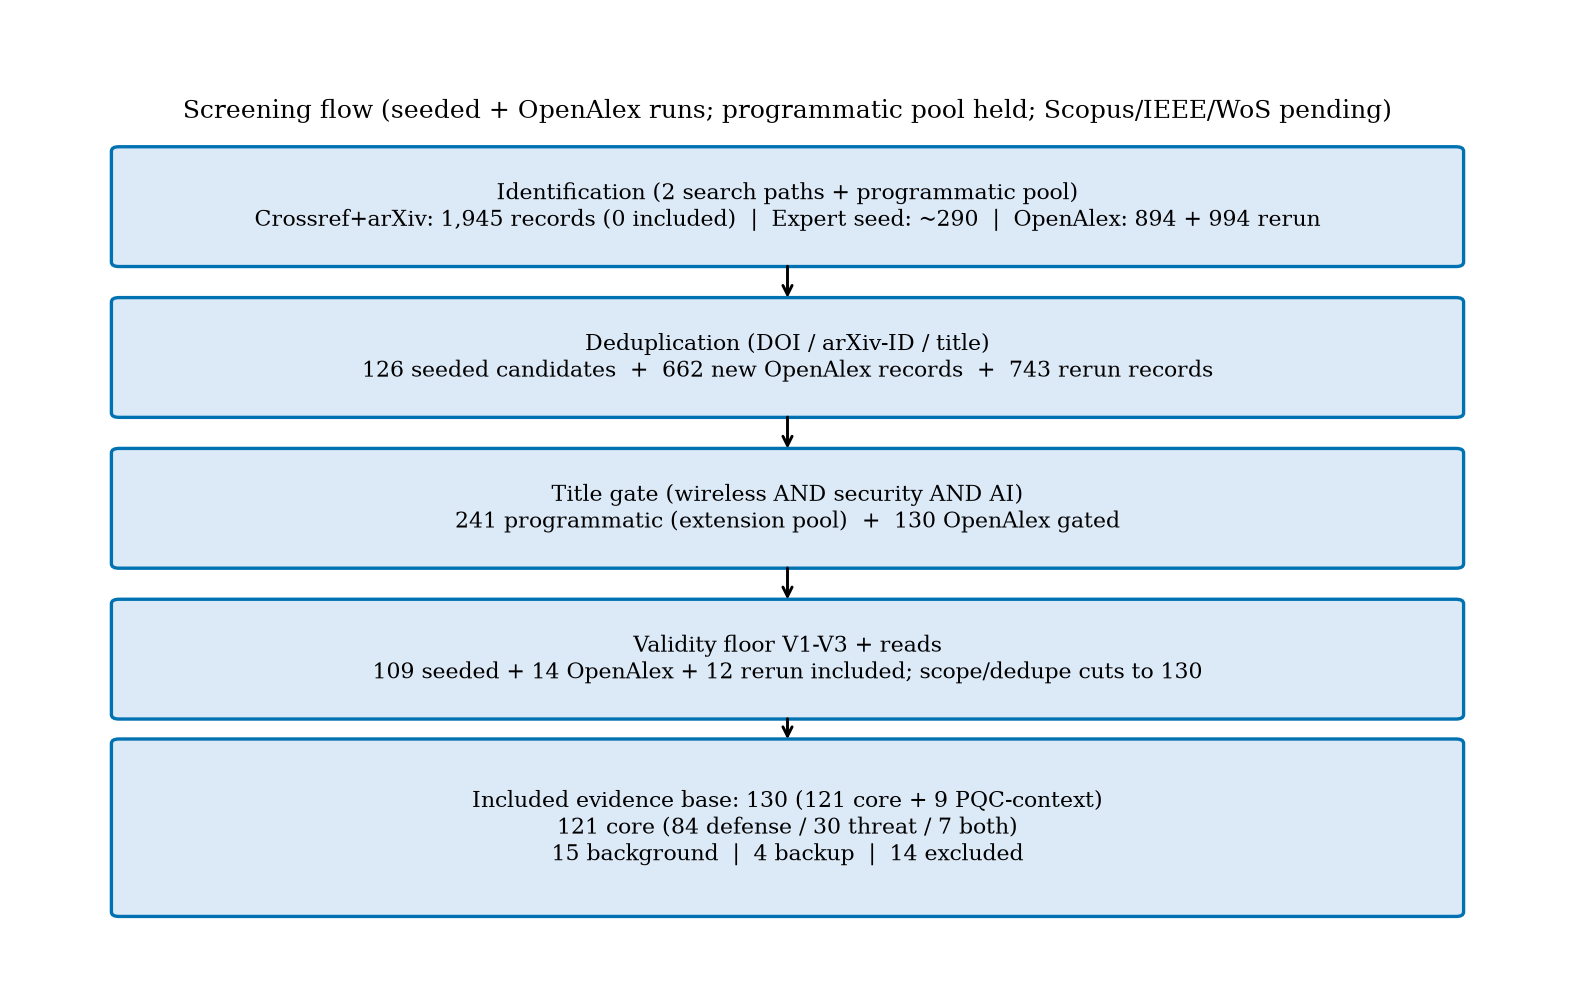
\includegraphics[width=0.92\linewidth]{figures/Fig1_screening_flow.png}
\caption{Study-selection flowchart. Programmatic records were retrieved from the Crossref and arXiv APIs (Path A, 241 gated extension-pool records released with disposition, not merged silently), OpenAlex database hits were deduplicated against them and title-gated (Path C), the expert-seeded path and two OpenAlex database runs were screened against the validity floor, an adjudication pass applied scope and dedupe cuts before the corpus froze at 130 studies (105 seeded $+$ 13 OpenAlex $+$ 12 rerun). Every record carries a verified resolvable identifier (see \S\ref{sec:intro}).}
\label{fig:flow}
\end{figure}

\subsection{Inclusion and exclusion criteria}
Table~\ref{tab:criteria} summarizes the criteria. Inclusion required: (i) radio-link/wireless population; (ii) security link (broad wireless-ML-security scope per \S\ref{sec:intro}: encryption, authentication including localization-fingerprint attacks where geofence bypass breaks an authorization boundary, key exchange/management/generation, physical-layer security, anti-jamming/secure communications, signal/traffic analysis where the classifier is the security boundary, side-channel analysis, federated privacy); (iii) AI involvement; (iv) dated 2020--2026, English, retrievable; (v) evaluable evidence (experiment, testbed, simulation, proof, cryptanalysis); (vi) peer-reviewed venue or reputable arXiv preprint (ID$+$version$+$access date; published supersedes; preprints $\le$40\%---observed 14.6\%). Exclusion: not wireless; no security link; no AI link; survey/opinion without primary mechanism (background only); pre-2020; non-English; retracted; unretrievable; duplicate (one same-team conference-to-journal extension deduped: T02 subsumed by T03; two same-team companion pairs counted as distinct records with disclosure---D55/T15 and D20/T20---each with a drop-one-pair sensitivity check); no evaluable evidence; preprint without evaluation. Adjudications logged: domain-informed cellular fuzzing without ML content is excluded for failing AI involvement (T07, consistent with the T24 exclusion); Wi-Fi localization-fingerprint attacks count where geofence bypass breaks an authorization boundary (T42 included on that ground, not on a forgery-breaks-authentication claim); signal-classifier attacks count where the classifier is the security boundary (T44 included under D36/D37 precedent); IoT traffic-classifier attack-plus-defense counts as dual-track protocol work (T46 included); wireless-FL-privacy work counts where the privacy guarantee is produced by channel properties (over-the-air superposition, channel-noise differential privacy)---a physical-layer mechanism under the D24 precedent---while generic FL-application papers without a channel-produced guarantee are excluded; acoustic/vibration SCA on PQC fails the radio-link population (T45 excluded to related work); Wi-Fi sensing without security link moved to background (including T34); 5G regression-robustness work without a security boundary excluded (T35); Xplore-hosted rows counted as peer-reviewed (Xplore hosts only peer-reviewed content), venue reverify at full-text read; author-claimed venues without proceedings records coded preprint (D26, T05-preliminary, D46-submitted, D48, P09-accepted), while author claims confirmed by a publisher record stay peer-reviewed (D41 TVT proceedings record, D52 TCCN proceedings record, T28 USENIX proceedings). Who screened/coded (all humans): Screener 1 performed 100\% title/abstract screening and full-text retrievability checks on every included record, with eligibility coding from full text where retrieved and from abstracts otherwise (110 rows abstract-only, including all 32 Unclear-source rows; 20 rows body-read as logged), plus 100\% charting; Verifiers A and B performed corrective checks on a 22-record sample (\texttt{verifier\_pack.csv}) with raw inclusion-disagreement 1/22 (4.5\%, 95\% exact interval roughly 0.1--23\%) on inclusion decisions only---it says nothing about coding reliability; blind R-score rescores were not completed; the reconciliation pass above was a single-coder rule-alignment, not a second coding. AI assistance was limited to candidate pooling, prose drafting, and copy-editing under human control---no screening, coding, or counting decision was delegated (see Declarations). No blind double-coding was completed, so no $\kappa$ is claimed---single-coder classification is a stated limitation and a 20--25\% blind double-code with Cohen $\kappa$ (binary) and quadratic-weighted $\kappa$/ICC(2,1) (R1--R5) remains future work. Bibliography verification (no IDs fabricated, none shared): every record carries a resolvable identifier checked against Crossref, arXiv, ACM, or USENIX; record-level corrections re-keyed D20 (true TVT paper) and D55 (true TCCN paper), corrected D31 year 2024$\rightarrow$2025 and T38 year 2021$\rightarrow$2022 to published versions, confirmed T03 (TMC 2026) and T28 (USENIX Security 2026 proceedings) as published, and recoded D48 to preprint (ICASSP per author comment only).

\begin{table}[tbp]
\centering
\caption{Inclusion and exclusion criteria applied during corpus screening.}
\label{tab:criteria}
\begin{tabular}{@{}p{2.2cm} p{5.5cm} p{6.0cm}@{}}
\toprule
Dimension & Included & Excluded \\
\midrule
Population & Radio-link/wireless systems & Wired-only, pure sensing without crypto link \\
Concept & Crypto primitive $+$ AI involvement & Missing either link \\
Document & Peer-reviewed $+$ reputable arXiv ($\le$40\%) & Surveys w/o mechanism, evidence-free preprints \\
Period & 2020--2026 & Pre-2020 \\
Verification & DOI/arXiv-ID resolved & Unresolvable, retracted, duplicate \\
Language & English & Non-English \\
\bottomrule
\end{tabular}
\end{table}

\subsection{Classification framework}
Each paper was classified along six fields: (1) security function (8 values: Authentication/RFFI, Key generation/distribution, Anti-jamming/secure comms, Protocol/traffic/cryptanalysis, PQC migration contextual, Federated/privacy-preserving FL, Learned primitives/crypto, Side-channel attack analysis); (2) AI method family (adversarial ML, deep supervised, PQC implementation, reinforcement/DRL, federated/private, traffic-analysis ML, LLM-assisted, defensive/robust ML, classical/Bayesian, optimization-based, dataset/benchmark, survey); (3) track (threat 30 / defense 84 / both 7 / pqc-context 9, with T05/T14 moved to dual-track under the develops-and-evaluates-both rule); (4) primary data source; (5) validation approach; (6) readiness R1--R5 with an explicit rubric---R1 (all): 0 absent / 1 implicit / 2 explicit attacker capability $+$ assumptions; R2 (all): 0 theory/proof/analysis without data evaluation / 1 controlled evaluation (simulation, reused datasets or traces, cross-domain protocols on collected data) / 2 author-conducted OTA/testbed demonstration or demonstrated real key recovery---as applied, simulation-only rows score 1 per the protocol rubric (an earlier pass that had downgraded confirmed-simulation rows to 0 stands reversed and logged; the mapping is asserted programmatically over all 130 rows with one documented override (T01: Standard-split validation with R2=2 for demonstrated over-the-air key recovery---without it the threat mean would read 1.50); R4 (all): 0 neither / 1 code OR data / 2 both or artifact-evaluated; R3 defense/learned-crypto/auth: 0 no cost / 1 latency OR energy $+$ HW target / 2 both $+$ HW target, attack papers N/A $+$ charted \texttt{attacker\_cost}; R5 defense/PQC-context: 0 none / 1 mentions 3GPP/IETF/NIST/ETSI / 2 evaluated against profile, attack papers N/A $+$ charted \texttt{affected\_standard}---each 0--2 with N/A handling (report medians/ranges per track with N/A rates; total $=$ sum of applicable items only). Papers take a single dominant value per field; conservative coding throughout (abstract-level except where full-text reads are logged in \texttt{fulltext\_reads.md}; 32 Unclear-source rows remain a stated limitation). R3/R5 are N/A for the 30 attack-only rows (coded 0 as placeholders, never pooled): R3 is reported over defense rows only (mean 0.19, median 0) and R5 over defense, dual, and PQC-context rows (means 0.07/0.14/0.56, medians 0/0/1). Each paper additionally carries a venue channel---journal (65), conference/workshop (46), or preprint (19)---coded from confirmed venue strings for the channel analysis in \S\ref{sec:sensitivity}. Verifiers A and B reviewed a 22-record sample correctively (raw inclusion-disagreement 1/22) rather than by blind double-coding---no agreement statistic is claimed, and counts should be read as one documented coding. The complete dataset is released as \texttt{dataset\_papers.csv} precisely so independent coders can check, correct, or extend it; a glossary of frequently cited corpus IDs accompanies the archive (\texttt{data/glossary.md}).

\subsection{Comparative synthesis approach}
Quantitatively, classification fields are aggregated into cross-tabulations---function by year, method by year, data, validation, readiness per track---that characterize the corpus as a sample (\S\ref{sec:corpus}); every figure and count was generated programmatically from the released dataset (see \texttt{code/}; \texttt{check\_consistency.py} gates export on sums and caption n-values). Qualitatively, the review synthesizes each function critically: what each cluster assumes, demonstrates, and where its support is thin (\S\S\ref{sec:threat}--\ref{sec:cross}). The methodology has limitations readers should weigh: open-web seeding favors notable work (the two OpenAlex yields---14 then 12 eligible---are reported as recall evidence with the caveat that the first run was incomplete: its FL query hit rate limits, so the ``14 papers missed by seeded search'' says more about seeded-search limits than about saturation); no formal stopping rule was applied---collection stopped after the rerun plus adjudication pass, and Path A contributed zero included records, so triangulation rests on the seeded and database paths with the programmatic pool held as backup; title-gate screening can miss nonstandard terminology; preprint inclusion adds recency at the cost of version instability (frozen by ID$+$version$+$date; 18 preprints, 13.8\%, sensitivity-checked); single-coder classification carries no reliability statistic (rubric above; blind $\kappa$ remains future work; raw inclusion-disagreement on the verifier sample was 1/22); full multi-registry triangulation is pending (Scopus/IEEE/WoS) with OpenAlex as executed substitute; 110 rows are coded from abstracts (including all 32 Unclear-source rows, concentrated in paywalled journals 23/32) and only 20 rows were body-read; body reads only ever upgraded scores, so all R3--R5 rates are lower bounds by construction, so Fig.~\ref{fig:validmix} and Table~\ref{tab:validation} mix coding depths---full-text rows skew simulation-heavy (5/20) relative to abstract-coded rows (13/110)---and full R3--R5 body reads remain future work. \S\ref{sec:corpus} should therefore be read as a structured sample, not a census---which is why this paper describes itself as a scoping review with bibliometric classification rather than a meta-analysis. No pooled effect sizes or significance tests are reported: metric heterogeneity (accuracy vs KGR vs secrecy rate vs attack-success rate) forbids pooling---a deliberate choice; function $\times$ validation cross-tabulations are descriptive, and the WIRELESS-AI-RC checklist is scored against the corpus descriptively in \S\ref{sec:gaps}.

\section{Corpus Overview and Six-Year Evolution}
\label{sec:corpus}
\subsection{Publication trend}
The corpus spans 2020--2026 with a rising but non-monotonic profile: 4 (2020), 17 (2021), 10 (2022), 21 (2023), 29 (2024), 36 (2025), 13 (2026 partial) (Figs.~\ref{fig:composition}--\ref{fig:years}). The 2021 bump is substantially a coverage effect: 5 of the 7 rerun-added FL-privacy papers date to 2021, without which the year reads 12. Excluding those 7 as a sensitivity check (N=123): defense R2 reads 1.32 instead of 1.27 while threat R2 is unchanged at 1.53, and simulation-only reads 16 instead of 18---the threat-realism lead, dual-track lowest realism, and RFFI dominance hold either way. Two caveats: the corpus is curated, so the curve partly reflects curation as well as field growth; and preprint share rises with recency, which is the velocity justification for their inclusion (\S\ref{sec:sensitivity}). With those caveats, the profile matches the field's post-2020 SDR-democratization and the 2024--2025 adversarial-ML surge. Sensitivity: dropping either duplicate-ID pair (D55/T15 or D20/T20) moves yearly totals by at most one paper and leaves the acceleration pattern unchanged.

\begin{figure}[tbp]
\centering
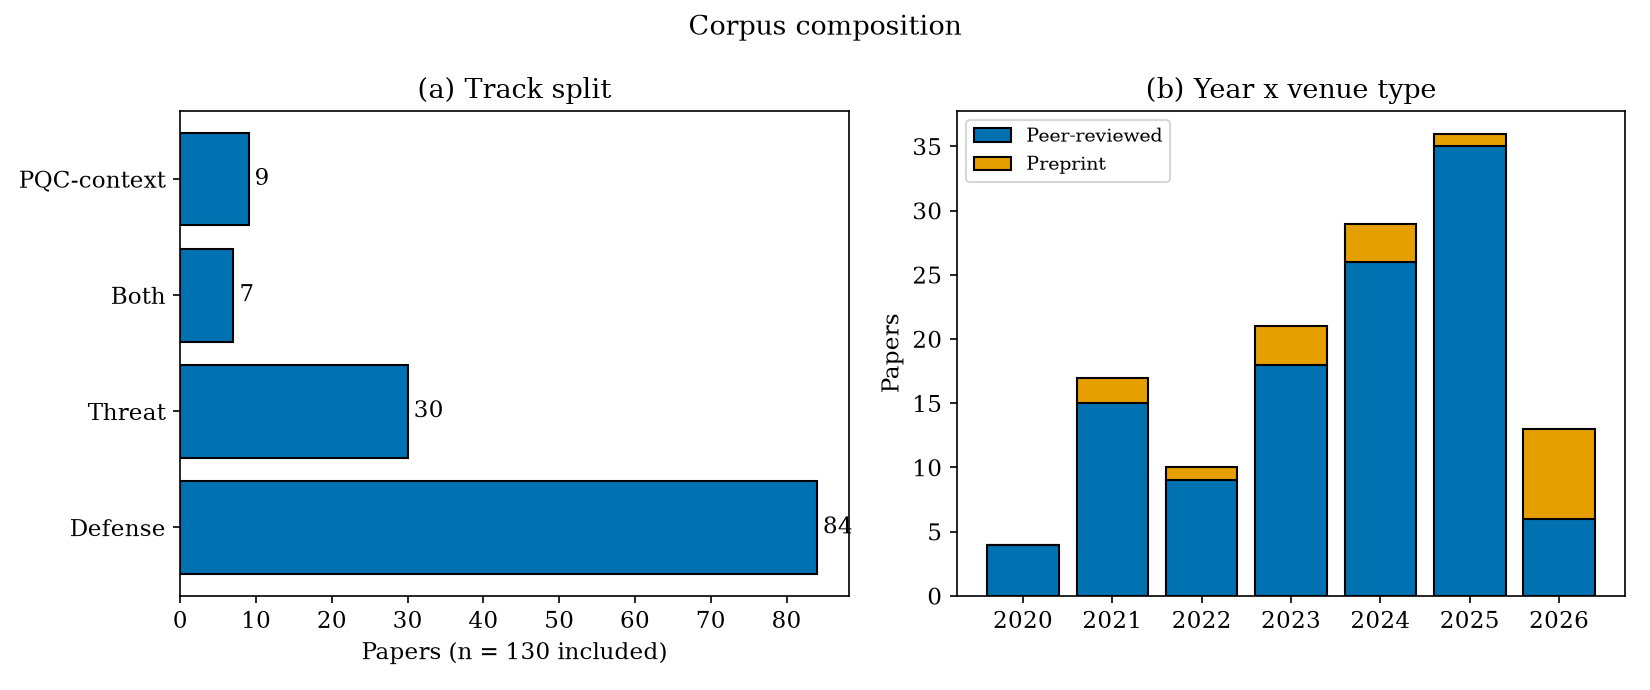
\includegraphics[width=0.95\linewidth]{figures/Fig2_corpus_composition.png}
\caption{Corpus composition: (a) track split (n=130); (b) year $\times$ venue type. Preprint share rises with recency.}
\label{fig:composition}
\end{figure}

\begin{figure}[tbp]
\centering
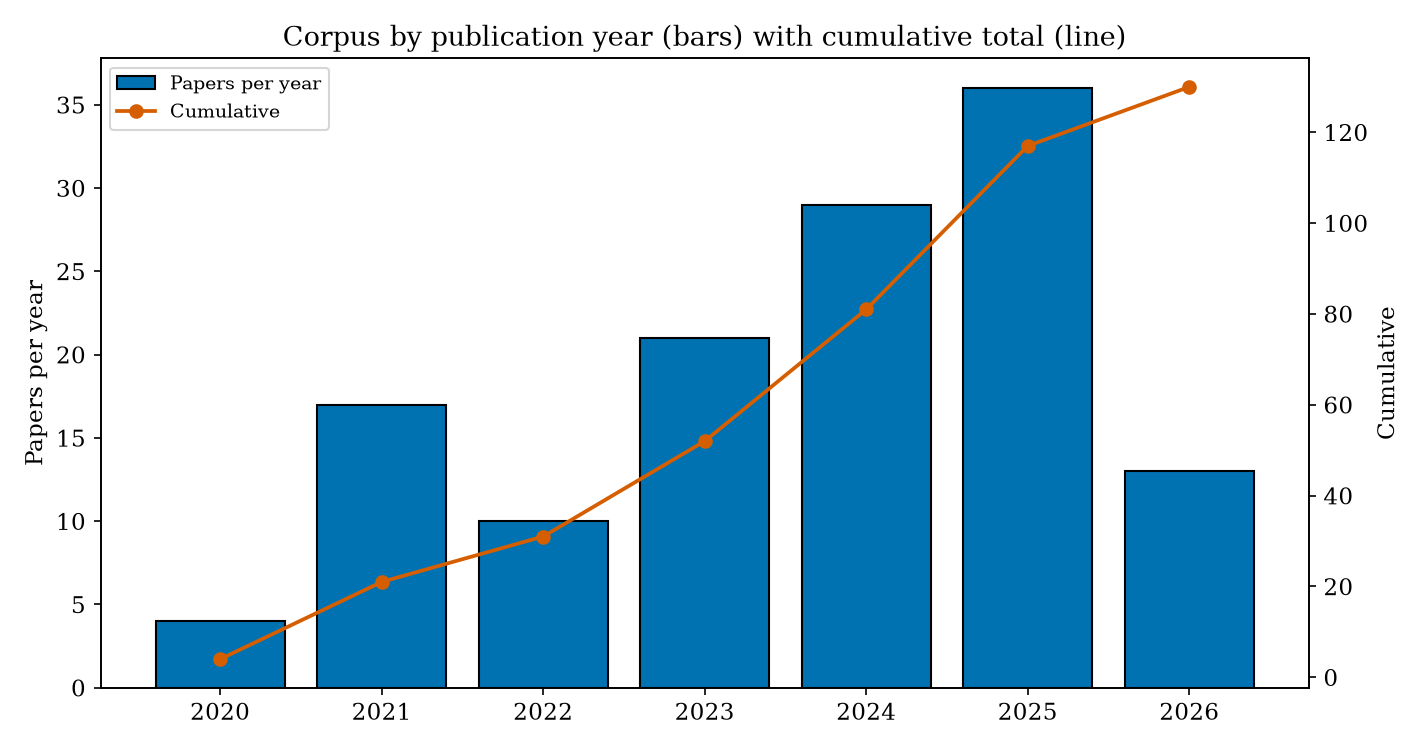
\includegraphics[width=0.92\linewidth]{figures/Fig4_year_trend.png}
\caption{Corpus composition by publication year (bars) with cumulative total (line). 2026 is a partial year.}
\label{fig:years}
\end{figure}

\subsection{Method-family evolution}
Deep supervised learning leads with 45 papers against 40 adversarial ML (Fig.~\ref{fig:methods}, Table~\ref{tab:methods}), a 5-paper margin that is not robust: the database-rerun merge added 4 deep-supervised RFFI papers while the dedupe cut removed two adversarial papers (T02 subsumed by T03; T35 excluded), and the federated-privacy additions sit in neither family. Deep supervised work led in every year through 2023 (2--1 in 2020 through 9--7 in 2023); 2024 is adversarial's peak year (11 papers) but not a permanent lead change, and 2026 stands 3--4. Deep supervised totals 21 papers through end-2023, and only 33 of its 45 address RFFI, so ``deep supervised fingerprinting'' mislabels the family (remainder: key generation 8, side-channel 2, anti-jamming 1, protocol/traffic 1). Adversarial ML spans white-box, black-box UAP, GAN-spoofing, backdoors, and universal PHY perturbations, with the 2025--2026 wave adding self-supervised-target backdoors [T41], over-the-air Wi-Fi attacks [T42], and frequency-selective strikes [T44]. Reinforcement/DRL holds at 9, all defense-side (anti-jamming, UAV relay, secrecy-rate optimization). PQC implementation (9) concentrates 2024--2026. Federated/private learning climbs to 12---nearly tripled by the rerun coverage correction, reported as such rather than as field growth---traffic-analysis ML (2), a single LLM-assisted fuzzer (ConSeT [T28], 2026), defensive/robust ML (2), dataset/benchmark contributions (2), survey/systematization (6), classical/Bayesian (1), and optimization-based (1) fill the long tail; protocol fuzzing/analysis leaves the taxonomy with T07's exclusion. The sole classical/Bayesian paper sits under RFFI. The families are not mutually exclusive in practice; dominant-family coding understates mixing.

\begin{table}[tbp]
\centering
\scriptsize
\setlength{\tabcolsep}{2pt}
\caption{Method families in the corpus: representative techniques, strengths, and limitations.}
\label{tab:methods}
\begin{tabular}{@{}>{\raggedright\arraybackslash}p{2.5cm} >{\raggedright\arraybackslash}p{0.9cm} >{\raggedright\arraybackslash}p{2.9cm} >{\raggedright\arraybackslash}p{2.9cm} >{\raggedright\arraybackslash}p{2.9cm}@{}}
\toprule
Method family & Papers & Techniques & Strengths & Limitations \\
\midrule
AdvML & 40 & FGSM/UAP, GAN-spoof, backdoor & Threat evidence; OTA-demo & Split 20 threat / 7 dual / 13 defense \\
DeepSup & 45 & CNN/RNN/Transf., open-set & Closed-set accuracy & Accuracy $\ne$ auth \\
PQC-impl & 9 & ML-KEM/ML-DSA, WKyber, LAKE & Onboard costs & Bandwidth blocks \\
DRL & 9 & Anti-jam power/relay & Adaptive control & Mixed grades (5 testbed); cost-silent \\
Fed/priv & 12 & DP-OTA-FL, robust aggregation & Privacy $+$ wireless-aware & Small scale; coverage-corrected \\
DataBench & 2 & Trace sets, open-set benchmarks & Reusable evidence & Rarely released \\
DefML & 2 & Robust training, unlearning & Adversary-aware training & Thin \\
TrafficML & 2 & Flow/classifier models & Deployed-boundary relevance & Evasion-prone \\
Survey & 6 & Reviews, maps & Maps field & No primary validation \\
Other & 3 & KNN/SVM, SCA/SDR, LLM fuzzing & Niche depth & Thin, scattered \\
\bottomrule
\end{tabular}
\end{table}

\begin{figure}[tbp]
\centering
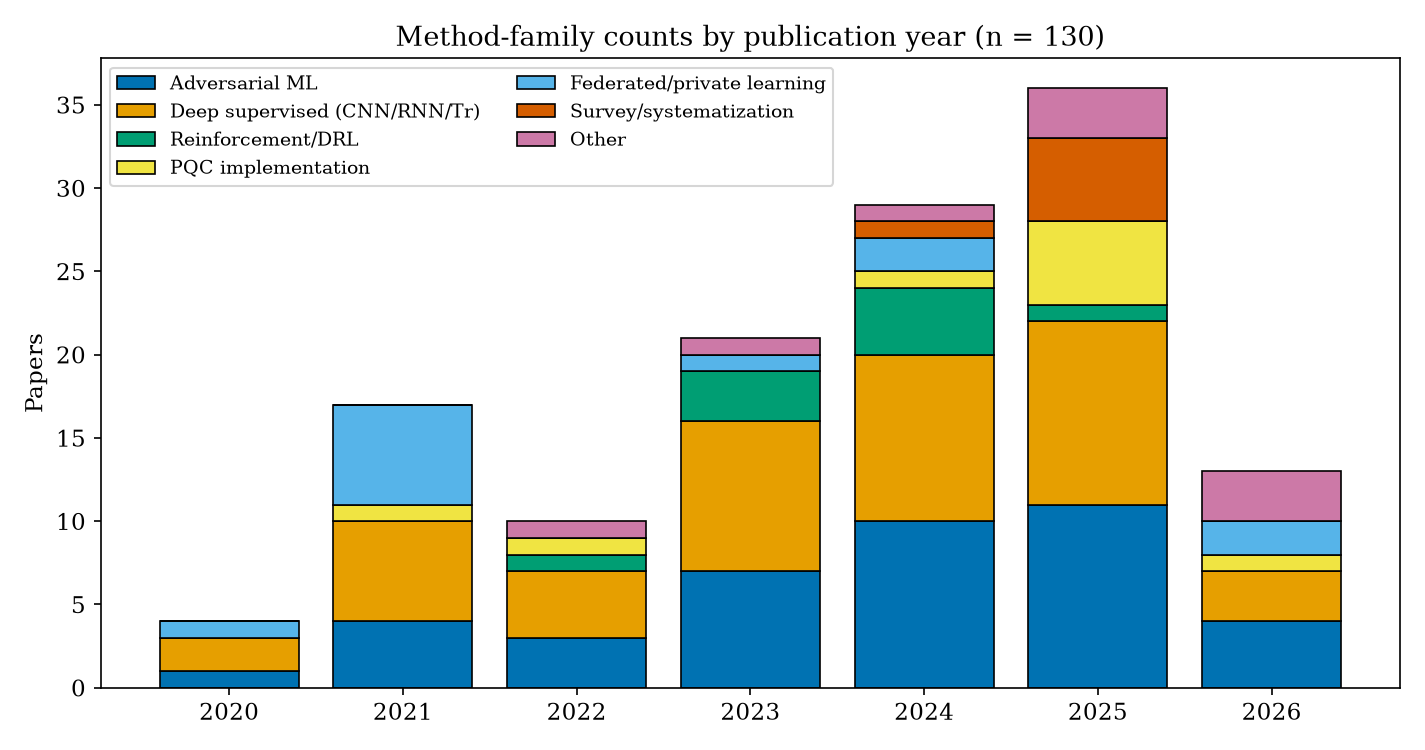
\includegraphics[width=0.95\linewidth]{figures/Fig5_method_by_year.png}
\caption{Method-family counts by publication year (n=130). Deep supervised learning led every year through 2023; 2024 is adversarial ML's peak year (11 papers), not a permanent overtake; 2026 stands 3--4.}
\label{fig:methods}
\end{figure}

Three observations qualify this trajectory. First, the families overlap in practice and dominant-family coding understates method mixing. Second, the adversarial rise is partly a response to the recognized brittleness of fingerprint classifiers under domain shift---but attack papers are, on average, evaluated no more stringently against adaptive defenses than defense papers are against adaptive attacks (\S\ref{sec:threat}), and no cited threat paper exploits domain shift as a standalone vector (T40 documents consistent cross-device misclassification under domain shift and demonstrates its use as a backdoor for system intrusion on real-world experiments---attack surface with a demonstrated trigger, not a deployed exploit). Third, the LLM-assisted cluster is too small to represent a trend; its significance is that LLM-based baseband analysis is appearing at all.

\subsection{Application-area distribution}
Functionally the corpus is dominated by Authentication/RFFI: 69 of 121 core (57.0\%), followed by Anti-jamming/secure comms (14), Key generation/distribution (12), Federated/privacy FL (11), Protocol/traffic/cryptanalysis (10), PQC-context (9), Learned primitives (3), Side-channel analysis (2) (Fig.~\ref{fig:heatmap}, Table~\ref{tab:functions}). The center of gravity sits in RFFI $\times$ (adversarial 27 $+$ deep-supervised 33)---deep supervised now leads inside RFFI as well as overall. By contrast, learned primitives (3) are thin---telling, since these are where cryptographic consequences are most direct. Cutting the same data by track (Fig.~\ref{fig:methodtrack}) sharpens the asymmetry that \S\S\ref{sec:threat}--\ref{sec:defense} develop: adversarial ML splits 20 threat / 7 dual / 13 defense across tracks (the dedupe moved two attack-plus-defense papers to dual-track), deep supervised learning remains predominantly a defense instrument (42 defense vs 3 threat), and all reinforcement learning in the corpus sits on the defense side. Method-by-track figures pool dual-track papers with threat for readability; the text always gives the three-way split (for adversarial ML: 20 threat / 7 dual / 13 defense).
\begin{figure}[tbp]
\centering
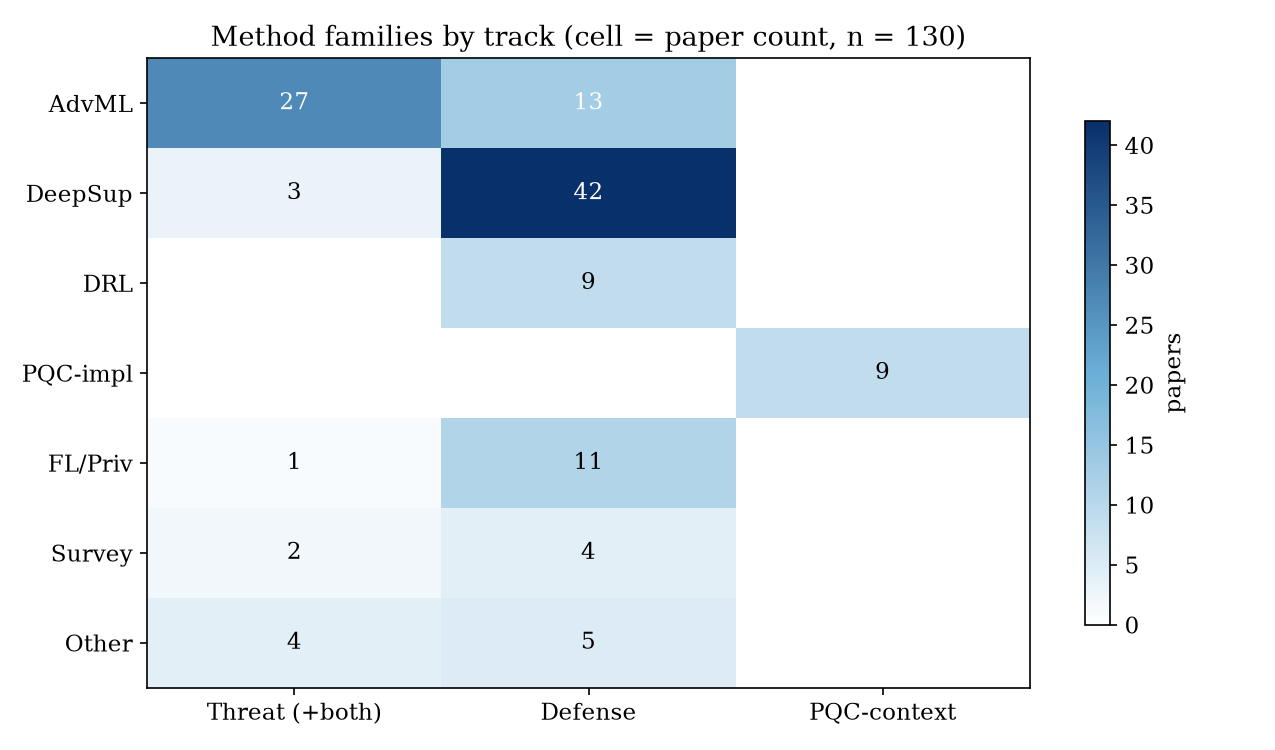
\includegraphics[width=0.85\linewidth]{figures/FigB_method_by_track.png}
\caption{Method families by track. Adversarial ML attacks; deep supervised learning defends; reinforcement learning is defense-only in this corpus.}
\label{fig:methodtrack}
\end{figure}

\begin{figure}[tbp]
\centering
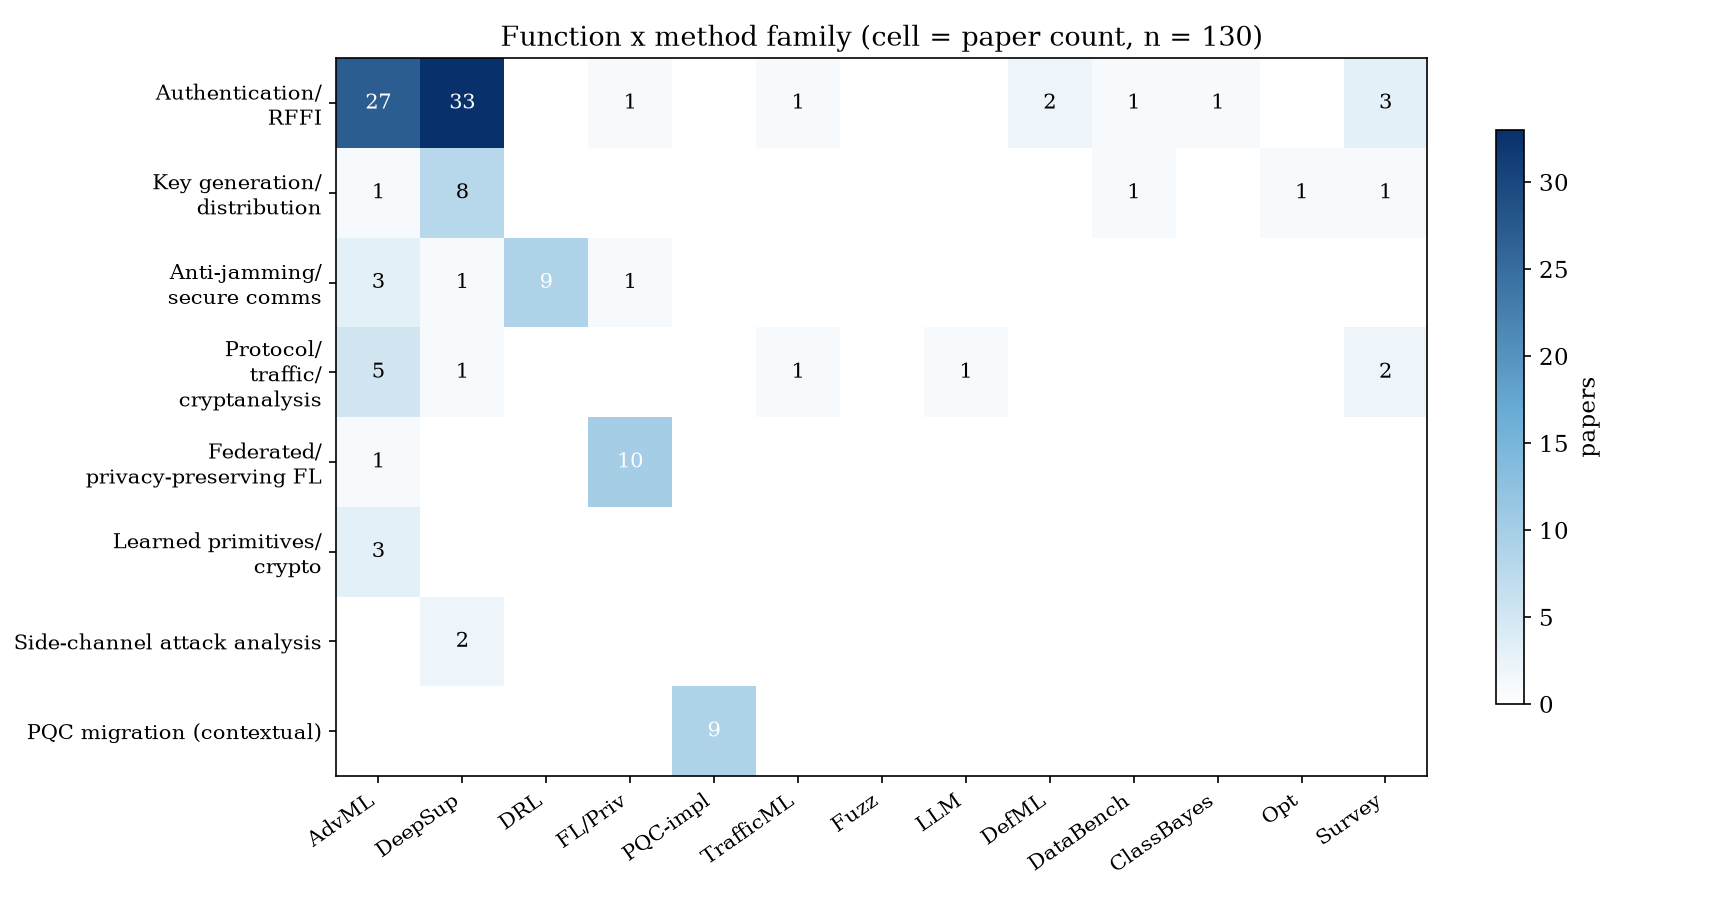
\includegraphics[width=0.95\linewidth]{figures/Fig3_function_method_heatmap.png}
\caption{The corpus mapped across security functions and AI method families (n=130). Cell values are paper counts.}
\label{fig:heatmap}
\end{figure}

\begin{table}[tbp]
\centering
\caption{Corpus composition: security function by publication year (130 papers). Machine-generated from the released dataset.}
\label{tab:functions}
\begin{tabular}{lrrrrrrrr}
\toprule
Function & '20 & '21 & '22 & '23 & '24 & '25 & '26 & Total \\
\midrule
Authentication/RFFI & 2 & 6 & 5 & 12 & 15 & 21 & 8 & 69 \\
Anti-jamming/secure comms & 0 & 0 & 2 & 3 & 6 & 3 & 0 & 14 \\
Key generation/distribution & 0 & 2 & 1 & 3 & 3 & 2 & 1 & 12 \\
Federated/privacy FL & 1 & 7 & 0 & 1 & 1 & 0 & 1 & 11 \\
Protocol/traffic/cryptanalysis & 0 & 0 & 1 & 2 & 2 & 3 & 2 & 10 \\
PQC migration (contextual) & 0 & 1 & 1 & 0 & 1 & 5 & 1 & 9 \\
Learned primitives & 0 & 1 & 0 & 0 & 1 & 1 & 0 & 3 \\
Side-channel analysis & 1 & 0 & 0 & 0 & 0 & 1 & 0 & 2 \\
Total & 4 & 17 & 10 & 21 & 29 & 36 & 13 & 130 \\
\bottomrule
\end{tabular}
\end{table}

\subsection{Data landscape and validation practice}
Data sources: Testbed/OTA measurement 46, Collected datasets/traces 26, Simulation 20, Analysis/benchmark 6, Unclear from abstract 32 (Fig.~\ref{fig:data}, left; data-source field, not validation). Validation: Testbed/field demonstration 47 (36\%), Cross-domain/generalization 26 (20\%), Simulation-only 18 (14\%), Standard split/unclear 35, Benchmark/analysis 4 (right panel). Crossing validation with track substantiates the headline (Fig.~\ref{fig:eval}): among threat papers (n=30), 16 are testbed/field demonstrations, 9 standard splits, 2 cross-domain, 2 simulation-only, 1 benchmark---measured plurality, not norm, with 8 threat data-sources unclear from abstract; key generation carries the simulation-only mass (7 of 12 keygen papers simulation-only; defense sim-only 16 of 84---Table~\ref{tab:funcval}). Readiness means per track (R3/R5 N/A for the 30 attack-only rows, coded 0 and never pooled): threat R1 1.70 / R2 1.53; defense R1 1.14 / R2 1.27 / R3 0.19 / R4 0.02 / R5 0.07; both (n=7) R1 1.86 / R2 1.14 (lowest realism); PQC-context R3 1.11 / R5 0.56---the only stratum with real cost and standards numbers (ESP32 DTLS 313~ms, sub-12~kB Dilithium, Cortex-M4 cycles; FIPS 203/186, 3GPP, 802.11, O-RAN references). Medians and N/A rates are reported with the rubric in \S\ref{sec:methods}: R3 median 0 on defense rows, R5 median 0 on defense and dual rows and 1 on PQC-context rows. Fig.~\ref{fig:readiness} plots the means by track (R1, R2, R4 for all tracks; R3/R5 for applicable tracks only). Table~\ref{tab:rdist} gives the underlying 0/1/2 count distributions (means are reported alongside, never alone), and Table~\ref{tab:ryear} shows readiness reporting by year: cost/artifact/standards reporting stays flat while output multiplies, even as validation grade improves by share---volume and maturity do not move together.

\begin{table}[tbp]
\centering
\footnotesize
\caption{Readiness-score count distributions (0/1/2) over all 130 rows. R3/R5 zeros include N/A placeholders for the 30 attack-only rows.}
\label{tab:rdist}
\begin{tabular}{@{}lccc@{}}
\toprule
Score & 0 & 1 & 2 \\
\midrule
R3 cost & 101 & 25 & 4 \\
R4 artifacts & 126 & 4 & 0 \\
R5 standards & 113 & 17 & 0 \\
\bottomrule
\end{tabular}
\end{table}

\begin{table}[tbp]
\centering
\footnotesize
\caption{Readiness means by publication year (n in parens): cost/artifact/standards reporting stays flat while output grows.}
\label{tab:ryear}
\begin{tabular}{@{}lccccccc@{}}
\toprule
 & 2020 (4) & 2021 (17) & 2022 (10) & 2023 (21) & 2024 (29) & 2025 (36) & 2026 (13) \\
\midrule
R3 mean & 0.00 & 0.29 & 0.10 & 0.24 & 0.28 & 0.25 & 0.38 \\
R4 mean & 0.00 & 0.00 & 0.00 & 0.00 & 0.00 & 0.09 & 0.08 \\
R5 mean & 0.00 & 0.12 & 0.10 & 0.05 & 0.17 & 0.14 & 0.23 \\
\bottomrule
\end{tabular}
\end{table}

\begin{table}[tbp]
\centering
\caption{Data sources recurring across the corpus.}
\label{tab:data}
\begin{tabular}{@{}>{\raggedright\arraybackslash}p{4.2cm} c >{\raggedright\arraybackslash}p{8.5cm}@{}}
\toprule
Data source & Papers & Typical use \\
\midrule
Testbed/OTA measurement & 46 & SDR captures, LoRa/Wi-Fi/UAV field demos \\
Collected datasets/traces & 26 & WiSig-style RFFI, RF-SCA trace sets \\
Simulation & 20 & Keygen channels, DRL jamming games, FL-privacy analysis \\
Analysis/benchmark & 6 & Proofs, systematizations, information-theoretic analyses \\
Unclear from abstract & 32 & Body-text resolution pending for paywalled rows (limitation; OA rows resolved where available) \\
\bottomrule
\end{tabular}
\end{table}

\begin{table}[tbp]
\centering
\caption{Validation practices across the corpus.}
\label{tab:validation}
\begin{tabular}{@{}>{\raggedright\arraybackslash}p{4.8cm} c >{\raggedright\arraybackslash}p{7.8cm}@{}}
\toprule
Validation & Papers & Interpretation \\
\midrule
Testbed/field demonstration & 47 & Deployment-relevant; threat-cluster plurality (16/30), not norm \\
Cross-domain/generalization & 26 & Strongest lab protocol; defense-cluster best (22/84) \\
Simulation-only & 18 & Model-fidelity dependent; keygen-heavy (7/12 keygen; 16/84 defense) \\
Standard split/unclear & 35 & Optimistic without isolation argument (9/30 threat) \\
Benchmark/analysis & 4 & No empirical validation (proof/analysis-grade); FL-privacy analyses \\
\bottomrule
\end{tabular}
\end{table}

\begin{table}[tbp]
\centering
\caption{Validation practice by security function (rows sum to function totals, n=130). Simulation-only work concentrates in key generation (7/12); RFFI is evaluated across all grades.}
\label{tab:funcval}
\begin{tabular}{@{}lccccc@{}}
\toprule
Function & Testbed & Cross-dom. & Sim-only & Std/unclear & Bench. \\
\midrule
Authentication/RFFI (69) & 21 & 22 & 4 & 22 & 0 \\
Anti-jamming/secure comms (14) & 8 & 1 & 4 & 1 & 0 \\
Key generation/distribution (12) & 3 & 1 & 7 & 1 & 0 \\
Federated/privacy FL (11) & 2 & 0 & 3 & 4 & 2 \\
Protocol/traffic/cryptanalysis (10) & 3 & 2 & 0 & 4 & 1 \\
PQC-context (9) & 5 & 0 & 0 & 3 & 1 \\
Learned primitives (3) & 2 & 0 & 0 & 1 & 0 \\
Side-channel analysis (2) & 1 & 0 & 0 & 1 & 0 \\
\bottomrule
\end{tabular}
\end{table}

\begin{figure}[tbp]
\centering
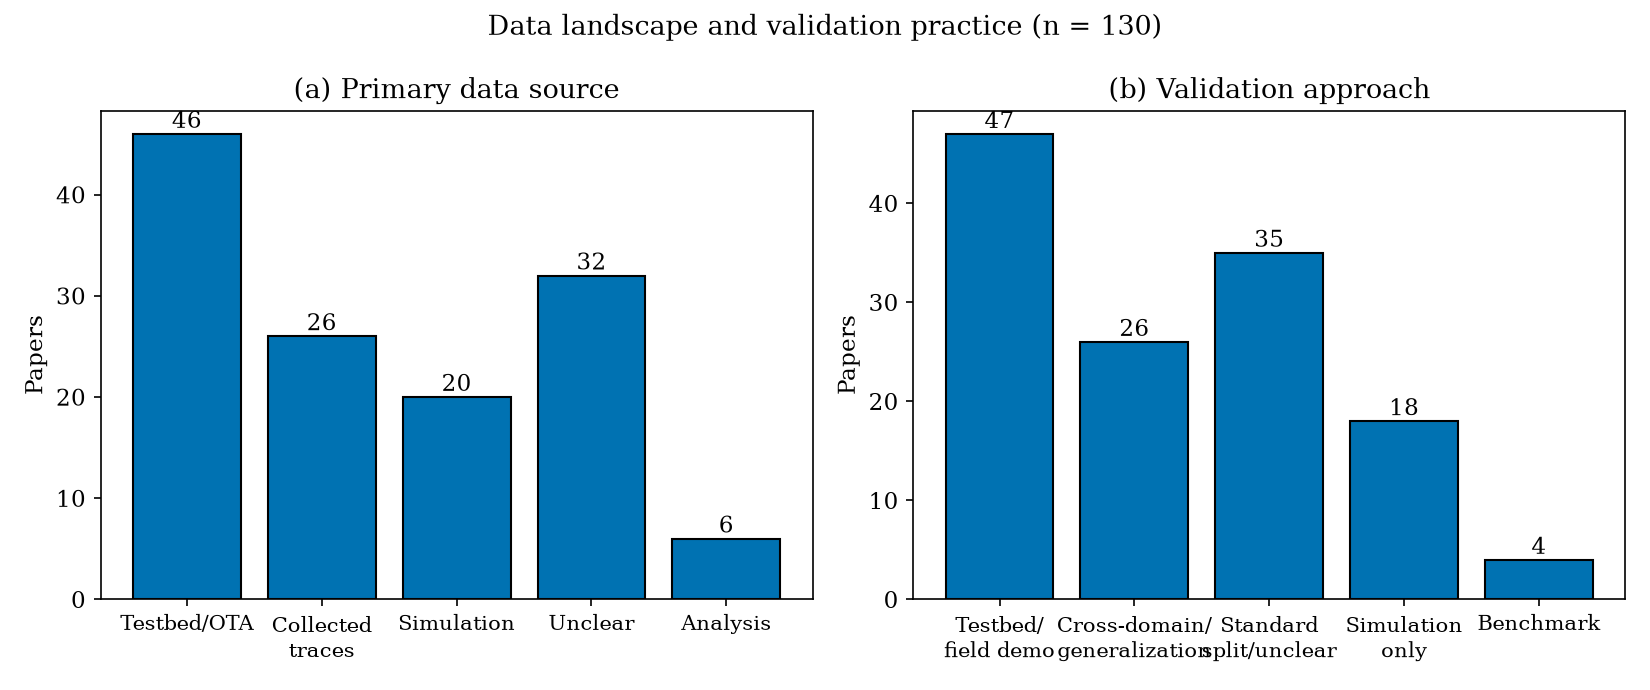
\includegraphics[width=0.95\linewidth]{figures/Fig6_data_validation.png}
\caption{Primary data sources (left) and validation approaches (right) across the corpus (n=130). Testbed/field demonstration is the modal validation; simulation-only work concentrates in key generation (7/12) with a smaller FL-privacy-analysis cluster.}
\label{fig:data}
\end{figure}

\begin{figure}[tbp]
\centering
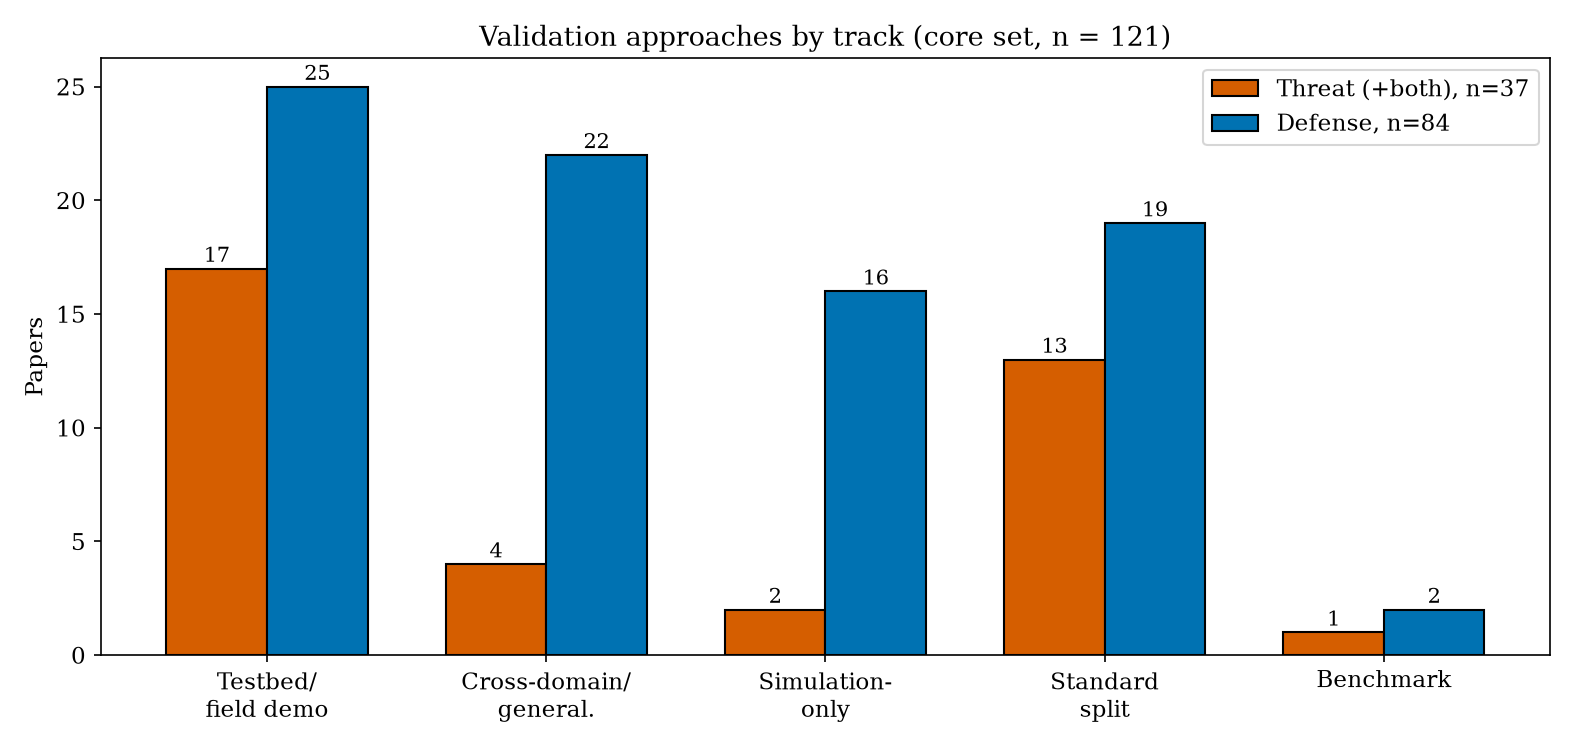
\includegraphics[width=0.95\linewidth]{figures/Fig7_eval_by_track.png}
\caption{Validation approaches by track (core set, n=121: 84 defense, 37 threat$+$both). Threat$+$both: 17 testbed/field, 4 cross-domain, 2 sim-only, 13 standard/unclear, 1 benchmark---measured plurality, not norm; defense carries the simulation-only mass (16 of 84). Data-source and validation fields are distinct---see text.}
\label{fig:eval}
\end{figure}

\begin{figure}[tbp]
\centering
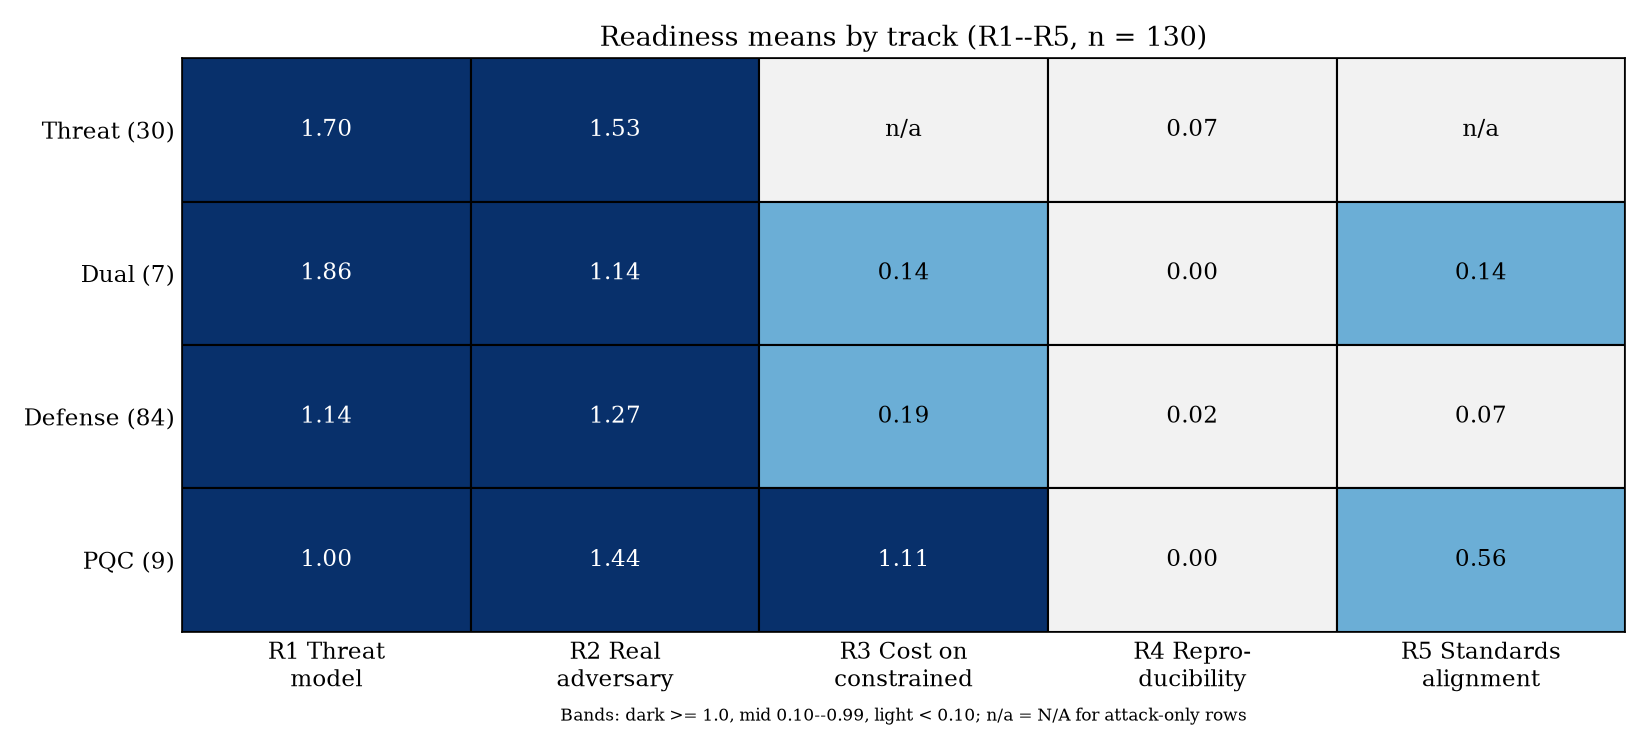
\includegraphics[width=0.95\linewidth]{figures/Fig8_readiness.png}
\caption{Readiness means by track (R1--R5, n=130; bands: dark $\ge$ 1.0, mid 0.10--0.99, light $<$ 0.10; n/a marks R3/R5 as N/A for attack-only rows; Dual row n=7). Threat work scores realism but releases almost nothing and aligns with no standards; only the PQC-context stratum reports real onboard costs.}
\label{fig:readiness}
\end{figure}

Reading these panels together yields the section's headline: the field's empirical base is bifurcated, not uniformly weak. Attacks are demonstrated; defenses are benchmarked. The year-by-year cut (Fig.~\ref{fig:validmix}) shows the evidence grade improving by share: testbed plus cross-domain work rises from about 40\% in 2021--22 to about 60\% in 2023--26 while simulation-only falls from about a quarter to under 10\%---though year arms hold only 10--35 papers each, so these shares are noisy, and absolute simulation-only counts hold roughly flat rather than being displaced.
\begin{figure}[tbp]
\centering
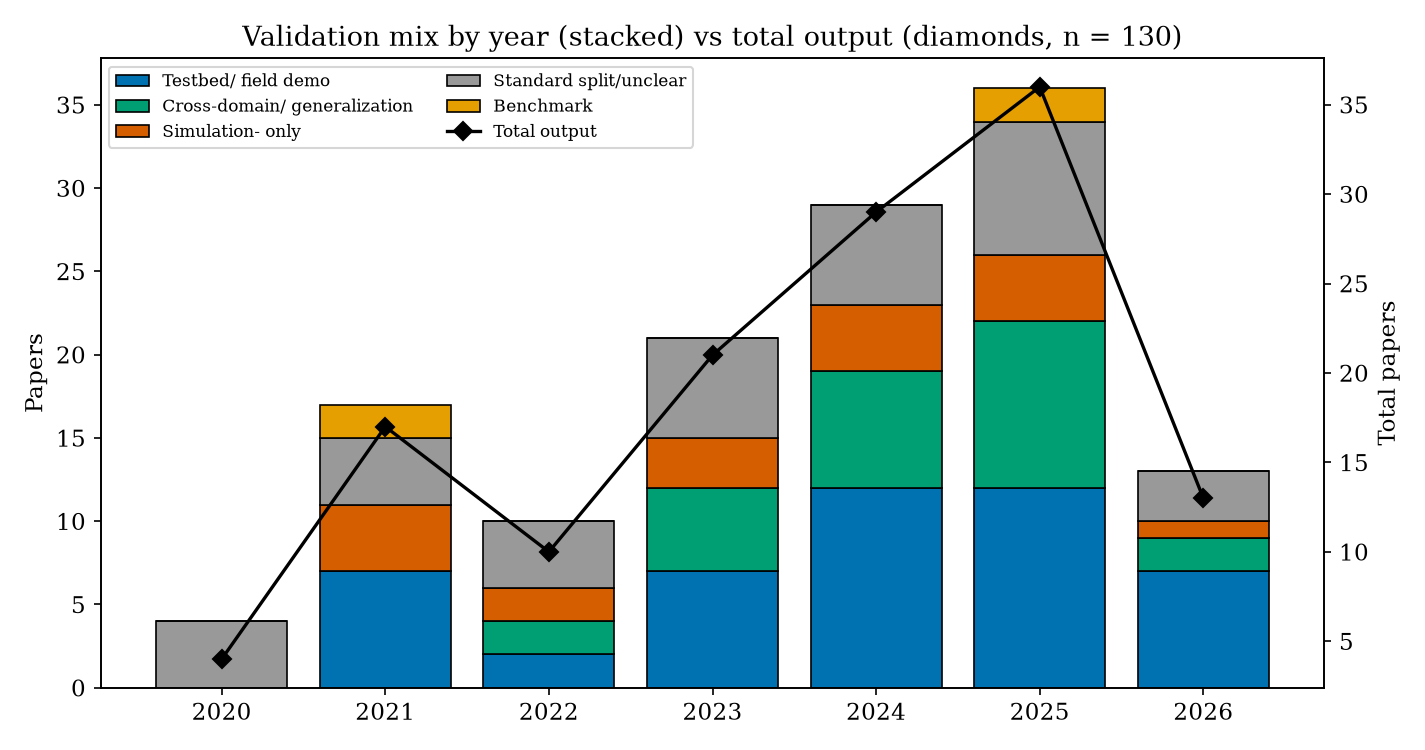
\includegraphics[width=\linewidth]{figures/FigA_validation_mix_by_year.png}
\caption{Validation mix by year (stacked) against total output (diamonds). Evidence grade improves by share (testbed plus cross-domain) while absolute simulation-only counts hold flat; year arms are n=10--35, so shares are noisy.}
\label{fig:validmix}
\end{figure}

\subsection{Sensitivity analysis: is peer review too slow for AI security?}
\label{sec:sensitivity}
Because the corpus mixes slow and fast publication channels---65 journal papers, 46 conference/workshop papers, and 19 preprints (venue channel coded from confirmed venue strings; \S\ref{sec:methods})---headline findings could in principle be a channel artifact. We therefore ask the question directly: do frontier methods appear first in fast channels, and does journal peer review compensate with stronger validation? The timing answer, within this verified sample, is partial; the rigor answer favors fast channels, noisily.

Frontier methods debut in fast channels, with stated exceptions. Conferences publish the first adversarial-ML paper in 2020 ([T39] WiseML) a year before the first journal one (2021); the first DRL paper in April 2022 ([D34] WCNC) a year before the first journal one (April 2023 [D22], earliest of the two 2023 journal DRL papers); deep-supervised work debuts tied in 2020 in both channels ([T01] ASHES workshop and the journal paper [D81])---[T01] is the first deep-supervised side-channel threat demonstration in-corpus, not the first fingerprinting paper. Journals lag conferences on adversarial-ML and DRL first appearance only (2 of 4 families); the PQC-context exception is noted (TCHES 2021 [P05] precedes the in-corpus ACNS 2022 PQC-wireless paper). Table~\ref{tab:firstappear} gives each cell with month granularity. The composition gap persists in shares: adversarial ML is 28\% of conference papers and 37\% of preprints but 31\% of journal papers (Fig.~\ref{fig:venue}, panel a; first-appearance map, panel b).

Journals lead conferences on both validation share (testbed 40\% vs 30\%) and mean evaluation-realism scores (R2 1.40 vs 1.26; preprints 1.32)---but both gaps are small relative to arm sizes (n=65/46/19), and the R2 gap is sensitive to single-coder judgment (reconciliation moved means by up to about 0.6), so no prestige gradient is claimed in either direction; the durable channel result is the timing lag, not a rigor ranking. Conferences lead journals by roughly a year on adversarial ML and DRL first appearance (deep-supervised debuts tied in 2020; PQC is reversed with a 2021 journal first). An earliest-public-date audit over all 15 DOI-year mismatches (Crossref online/print dates) moves no first-appearance cell---the D22 TVT paper printed April 2023 despite its 2022 DOI number, and D36's own arXiv dates to April 2021---so the lags stand under both issue-year and earliest-date coding; only P05 shifts (December-2020 online-first vs 2021 issue), which widens the PQC reversal. The preprint stratum (37\% testbed, heavily selected---see caveats) cannot carry a channel claim on its own. Consistent with the no-formal-tests rule (\S\ref{sec:methods}), no significance tests are run on these splits.

\begin{table}[tbp]
\centering
\footnotesize
\caption{First-appearance papers by method family and channel, with issue, online-first, and arXiv-v1 months where evidenced. Lags stand under both issue-year and earliest-date coding except P05 (Dec-2020 online-first vs 2021 issue).}
\label{tab:firstappear}
\begin{tabular}{@{}l l l l@{}}
\toprule
Family & Conference cell & Journal cell & Preprint cell \\
\midrule
Adversarial ML & T39 WiseML, Jul 2020 & T09 TCCN, Mar 2021 (D36 Mar 2022; arXiv Apr 2021) & T47 arXiv Jan 2022 \\
Reinforcement/DRL & D34 WCNC, Apr 2022 & D22 TVT, Apr 2023 (no online-first record) & --- \\
Deep supervised & T01 ASHES, Nov 2020 & D81 IEEE Access 2020 & D63 arXiv Jun 2023 \\
PQC implementation & P10 LNNS 2025 & P05 TCHES 2021 issue (online Dec 2020) & --- \\
\bottomrule
\end{tabular}
\end{table}

\begin{table}[tbp]
\centering
\caption{Venue-channel sensitivity: validation mix across journals (n=65), conferences (n=46), and preprints (n=19). Machine-generated from the released dataset.}
\label{tab:sensitivity}
\begin{tabular}{llll}
\toprule
Validation & Journal & Conference & Preprint \\
\midrule
Testbed/field demonstration & 26 (40\%) & 14 (30\%) & 7 (37\%) \\
Cross-domain/generalization & 13 (20\%) & 11 (24\%) & 2 (11\%) \\
Simulation-only & 6 (9\%) & 8 (17\%) & 4 (21\%) \\
Standard split/unclear & 20 (31\%) & 10 (22\%) & 5 (26\%) \\
Benchmark/analysis & 0 & 3 (7\%) & 1 (5\%) \\
\bottomrule
\end{tabular}
\end{table}

\begin{figure}[tbp]
\centering
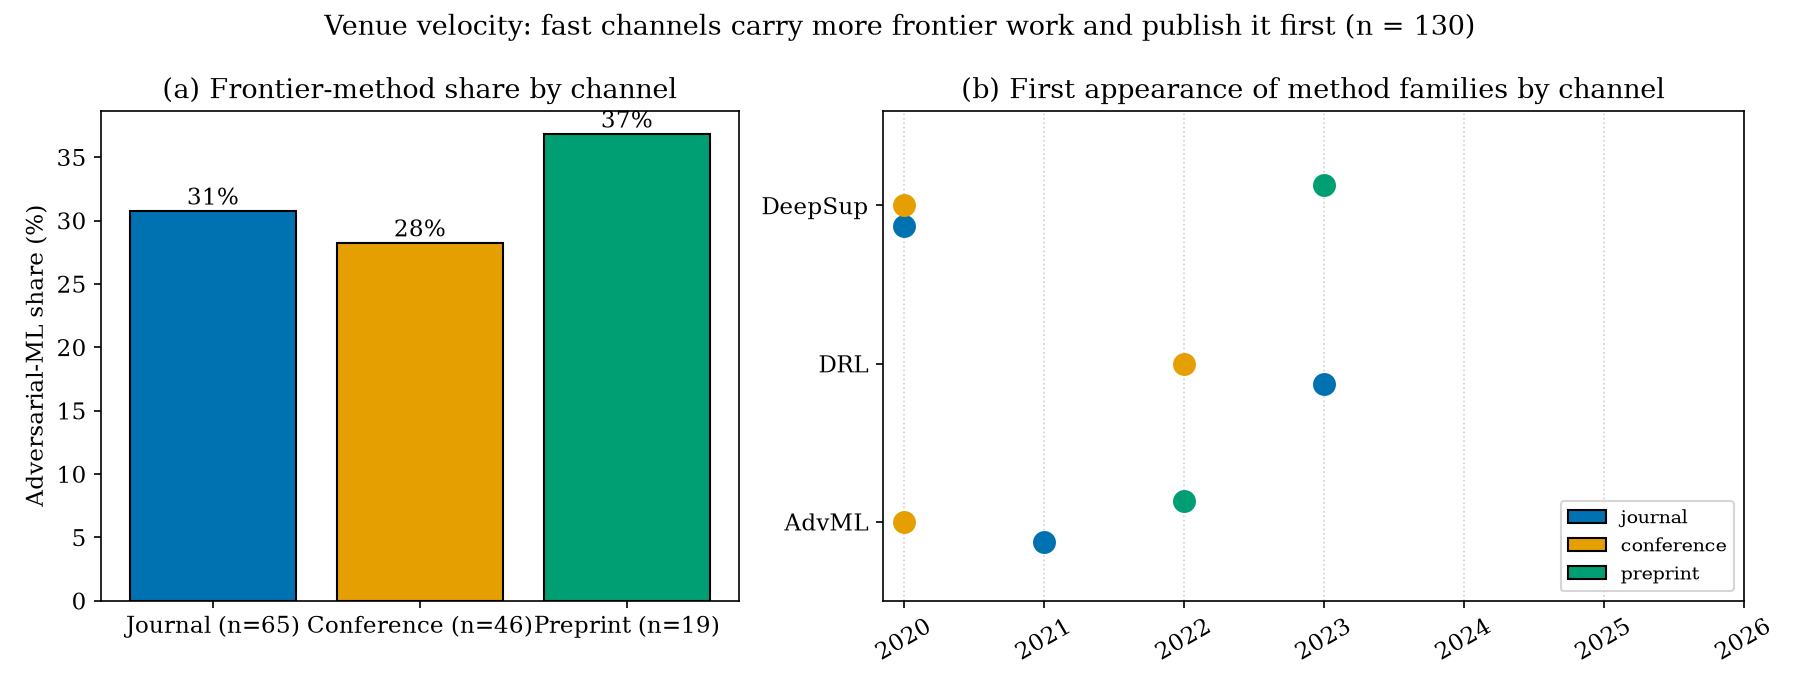
\includegraphics[width=\linewidth]{figures/FigE_venue_velocity.png}
\caption{Venue velocity. (a) Adversarial-ML share is highest in preprints (37\%), then journals (31\%), lowest in conferences (28\%). (b) First appearance of method families by channel: conferences lead journals on adversarial ML and DRL; deep-supervised debuts tied in 2020; PQC-context exception noted in text (TCHES 2021 precedes ACNS 2022). Dots jittered vertically where channels share a year.}
\label{fig:venue}
\end{figure}

Three caveats bound this finding, and the third is the most serious. First, the preprint arm is small (n=19), the conference arm mixes full conferences with workshops, and each first-appearance cell rests on a single paper in a curated sample at year granularity, so both the shares and the lags carry wide uncertainty. Second, the LLM-assisted family has a single published paper (USENIX Security 2026 [T28]) and cannot support any channel claim. Third, seeded expert search favors notable, well-evidenced preprints---weak preprints are never found or shortlisted---so the preprint stratum's scores partly reflect selection, not the channel. What selection cannot explain is the journal side of the ledger: journals trail conferences by roughly a year on adversarial ML and DRL first appearance while running close on validation (testbed 40\% vs 30\%; R2 1.40 vs 1.26). For a field where the adversary reads arXiv, that lag is a deployment-relevant result in itself---and it strengthens, rather than weakens, the case for the reporting checklist in \S\ref{sec:gaps}, since speed without standards is how the validation gap in \S\ref{sec:corpus} reproduces itself.

\section{AI-Enabled Threats: What the Corpus Demonstrates}
\label{sec:threat}
RFF/authentication attacks form the densest cluster (Table~\ref{tab:representative}): white-box FGSM/PGD and black-box UAP at 81.7\% with $\sim$no victim knowledge on real LoRa captures [T03], RL impersonation at $>$90\% from binary feedback [T18], GAN-spoofing at 76\% PHY-auth pass [T09], backdoors surviving Neural Cleanse/STRIP [T12] and working model-agnostically [T16], self-supervised-target backdoors [T41], over-the-air Wi-Fi attacks [T42], and fingerprint erasure as privacy attack [T06]. EM/RF side-channels move key recovery over the air at meters: BLE AES-128 at 15~m from $<$400 traces [T01], nRF AES-CCM at 1~m [T08], BLE re-keying LTK leakage in $\sim$30 traces. Protocol/traffic attacks show the stack above PHY is equally exposed: padding/shaping defeated by packet-size distributions [T19], and LLM-assisted semantic baseband fuzzing (ConSeT: 7 vulns including 3 CVEs across 542 phone models, plus 29 OAI-UE crash sites, USENIX Security 2026 [T28]). Critical assessment: attacks are evaluated against real systems with stated---often weak but honest---threat models (strong R2, narrow R1). The missing attack science is adaptive-defense evaluation: most stop at undefended classifiers, which is why Magmaw [T30] matters---it survives adversarial training, subtraction, detection, and oracle defenses. Domain shift is attack surface, not demonstrated exploit: no cited threat paper exploits shift as a standalone vector.

\begin{table}[tbp]
\centering
\footnotesize
\setlength{\tabcolsep}{3pt}
\caption{Representative corpus studies by function and method family. Entries gloss each study as: study summary (data basis; headline contribution).}
\label{tab:representative}
\begin{tabular}{@{}>{\raggedright\arraybackslash}p{2.4cm} >{\raggedright\arraybackslash}p{2.4cm} >{\raggedright\arraybackslash}p{9.2cm}@{}}
\toprule
Function & Family & Representative studies \\
\midrule
RFF/auth attack & Adversarial & White-box FGSM/PGD plus black-box UAP 81.7\% on LoRa captures (CNN/LSTM/GRU; no victim knowledge) [T03]; RL impersonation $>$90\% (SDR; binary feedback) [T18]; GAN-spoof 76\% (OTA; PHY-auth pass) [T09]; SSL-target backdoor [T41]; FooLoc OTA WiFi geofence-bypass [T42] \\
Side-channel & Deep supervised & Far-field BLE AES-128 at 15~m, $<$400 traces (OTA) [T01]; nRF AES-CCM at 1~m (RF-SCA) [T08]; BLE LTK in $\sim$30 traces \\
Protocol/traffic & Fuzzing/ML & LLM baseband fuzzing, 3 CVEs (phones; ConSeT) [T28]; padding defeat (traces; traffic-shape exploit) [T19] \\
Universal PHY & Adversarial & Magmaw, NDSS'25 (SDR; protocol-agnostic UAP vs encrypted link) [T30] \\
Defense RFFI & Robust/open-set & Contrastive, receiver-agnostic, open-set/few-shot, cross-receiver calibration [D75], multi-distance [D73], satellite PLA [D71] (captures; accuracy under shift) \\
Keygen & Deep/DRL & KDR/KGR improvements (mostly simulation; reciprocity $+$ IRS/relay) \\
Anti-jamming & DRL $+$ testbed UAV & Relay/power/secrecy-rate control (mixed: 8 testbed, 4 sim-only; costs mostly unreported) \\
PQC-context & Implementation & ML-KEM DTLS 313~ms on ESP32 (hardware; compute fine, bandwidth blocks); WKyber/LAKE (bandwidth attacks) [P08][P11] \\
AI$\times$PQC join & --- & Empty in-corpus (non-radio proximity study excluded; recorded gap) \\
\bottomrule
\end{tabular}
\end{table}

\section{AI-Assisted Defenses: What the Corpus Demonstrates}
\label{sec:defense}
RFF/PLA defenses chase domain shift: contrastive embeddings, receiver-agnostic training, open-set/few-shot enrollment, cross-receiver calibration [D75], multi-distance generalization [D73], domain-adaptive features [D72], satellite fingerprinting [D71], proactive authentication---accuracy under shift, rarely under attack. Key generation defenses improve KDR/KGR mostly in simulation, with a 2026 channel-informed neural scheme [D74] grounding features in over-the-air channel soundings. DRL anti-jamming optimizes relay/power/secrecy-rate without onboard-cost reporting. Federated privacy proves differentially private OTA aggregation at small scale. Critical assessment: the wall between \S\ref{sec:threat} and this section is the finding---dual-track studies are 7 of 130 (5.4\%; 7 of 121 core, 5.8\%), and dual-track realism runs lowest (mean R2 1.14 vs 1.53 threat, 1.27 defense---a 0.13 margin at n=7, so a descriptive remark, not a ranking claim), so closed-loop evaluation exists but is least realistic. RFF accuracy $\ne$ authentication; domain-shift misclassification is attack surface (T40), not demonstrated exploit. The defense literature's strongest protocols (cross-receiver, cross-day, open-set) are exactly the threat literature's attack surface.

\section{Quantum-Era Context (Separate Stratum)}
\label{sec:pqc}
Compute is feasible on ESP32/Pi-class hardware (ML-KEM DTLS 313~ms, beating classical baselines; sub-12~kB Dilithium; Cortex-M4 cycle counts); bandwidth expansion is the blocker; WKyber [P08] and LAKE [P11] attack exactly that. Short-range radio key-recovery evidence (far-field BLE SCA [T01]) shows keys can be pulled over the air, but no in-corpus paper addresses store-now-decrypt-later against the PQC transition for wireless fleets. The AI-threat $\times$ PQC join is empty: no in-corpus paper mounts ML-driven cryptanalysis of a PQC implementation over a radio link (an acoustic--vibration proximity study was excluded for failing the radio-link population; see \S\ref{sec:methods}). The join is recorded as an explicit gap (\S\ref{sec:gaps}), and the stratum stays separate as thesis hygiene requires.

\section{Cross-Cutting Directions}
\label{sec:cross}
Closed-loop evaluation---defined here as dual-track studies (7 of 130) plus any threat paper that evaluates against a stated defense and any defense paper that evaluates against a stated attack---reaches at least 14 of 121 core (11.6\%, a lower bound---abstract wording may hide further cases; a full-text audit is future work): the 7 dual-track papers (D08, D36, D37, T05, T11, T14, T46---5 under a stricter title-only dual rule with T05/T14 reverting to threat; T31 stays threat either way since its mitigation is secondary), 3 threat papers that demonstrate against defenses (T30 against adversarial training, subtraction, detection, and oracle defenses; T12 by bypassing Neural Cleanse and STRIP; T31 assessing a distillation defense on an OTA O-RAN testbed), and 4 defense papers that demonstrate against attacks (D67 against GAN-based impersonation; D54 against Byzantine poisoning; D32 against live impersonating UAVs; D48 flagging evasive queries). The broader measure remains the exception (the \S\ref{sec:threat}--\S\ref{sec:defense} wall), autonomous trust (real-time deadlines unbenchmarked; OTA crypto-agility essentially unaddressed; multi-agent trust in 1--2 papers while FL-for-drones falls to deauth$\rightarrow$impersonation chaining [T36]), and reproducibility (4 verified artifact releases among 121 core, 3.3\%) are the three cross-cutting threads (Fig.~\ref{fig:gaps}). Dual-track realism is lowest (mean R2 1.14, n=7---a 0.13 margin over defense, fragile at this n), which complicates any closed-loop optimism: evaluation exists but is least realistic. Function $\times$ validation cross-tabulations are descriptive (no significance tests; metric heterogeneity forbids pooling). The field optimizes estimators while adversaries optimize exploitability---a mismatch no single-function advance can fix. A venue-community check does not explain the asymmetry away: stratifying R2 by security venues (NDSS, CCS, USENIX, TIFS, WiseML and kin) versus comms and other venues, comms-venue threats outscore comms-venue defenses on realism (means 1.61 vs 1.31, n=23/68), while security-venue papers score lower in both tracks (threat 1.29, n=7---T01, T19, T20, T23, T28, T30, T39, of which T01, T28 and T30 score 2 and the analysis/workshop remainder scores 0--1; defense 1.12, n=16)---small-n and caution-worthy, but running against the community-norms confound rather than with it. Fig.~\ref{fig:layered} stacks the corpus by layer to make the coverage gap visible: the signal layer is contested, the link layer half-defended, the protocol layer thinly covered, and the system layer essentially absent.
\begin{figure}[tbp]
\centering
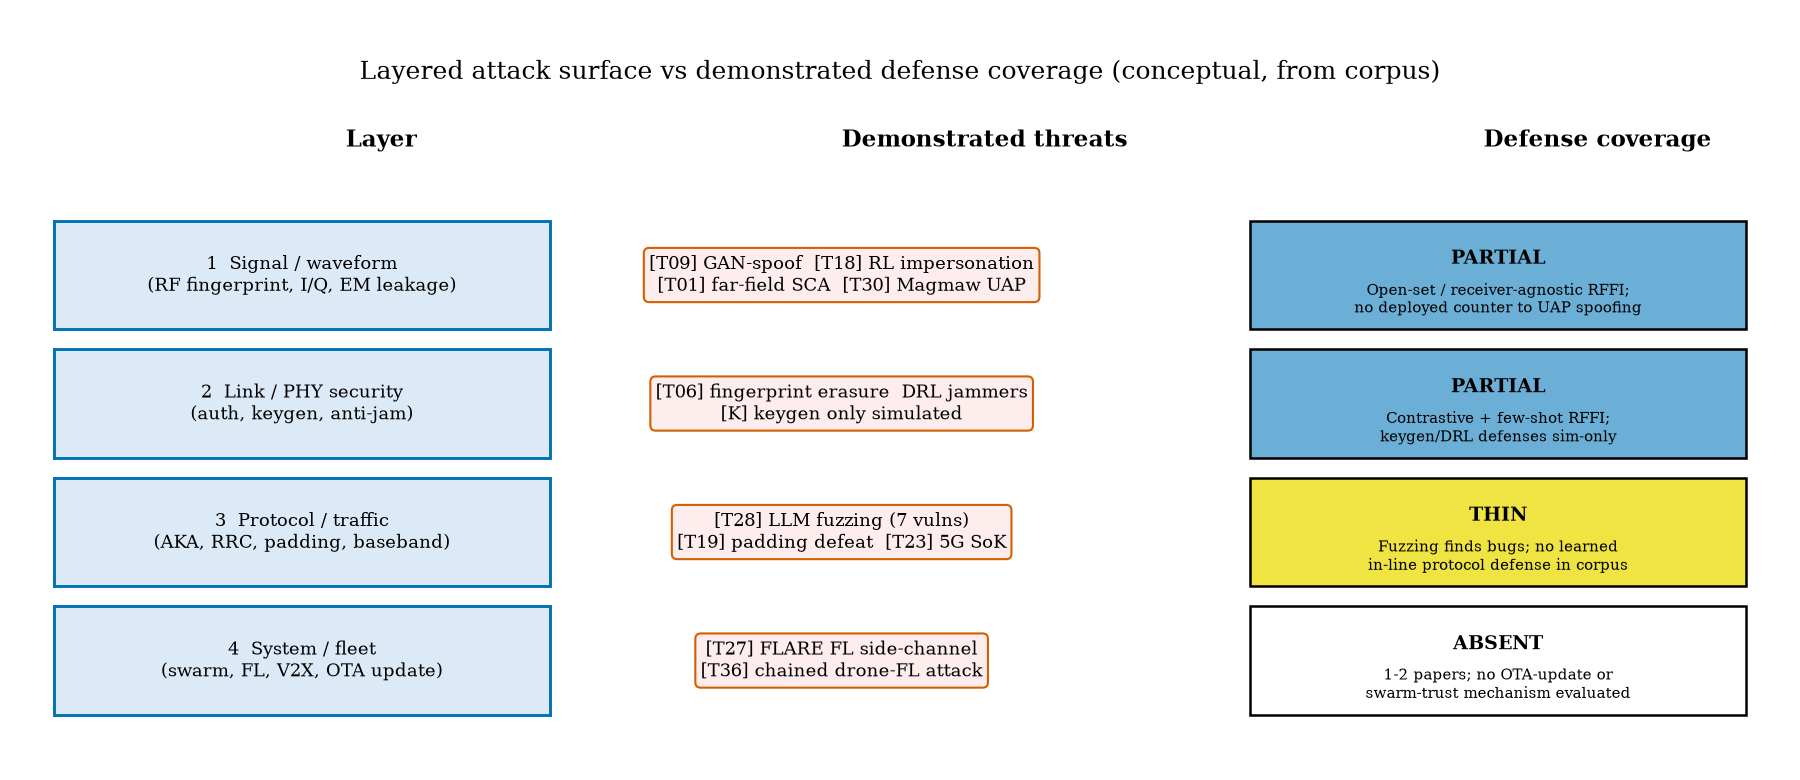
\includegraphics[width=\linewidth]{figures/FigD_layered_coverage.png}
\caption{Layered attack surface versus demonstrated defense coverage, synthesized from the corpus (conceptual). Coverage thins with every step up the stack.}
\label{fig:layered}
\end{figure}

\begin{figure}[tbp]
\centering
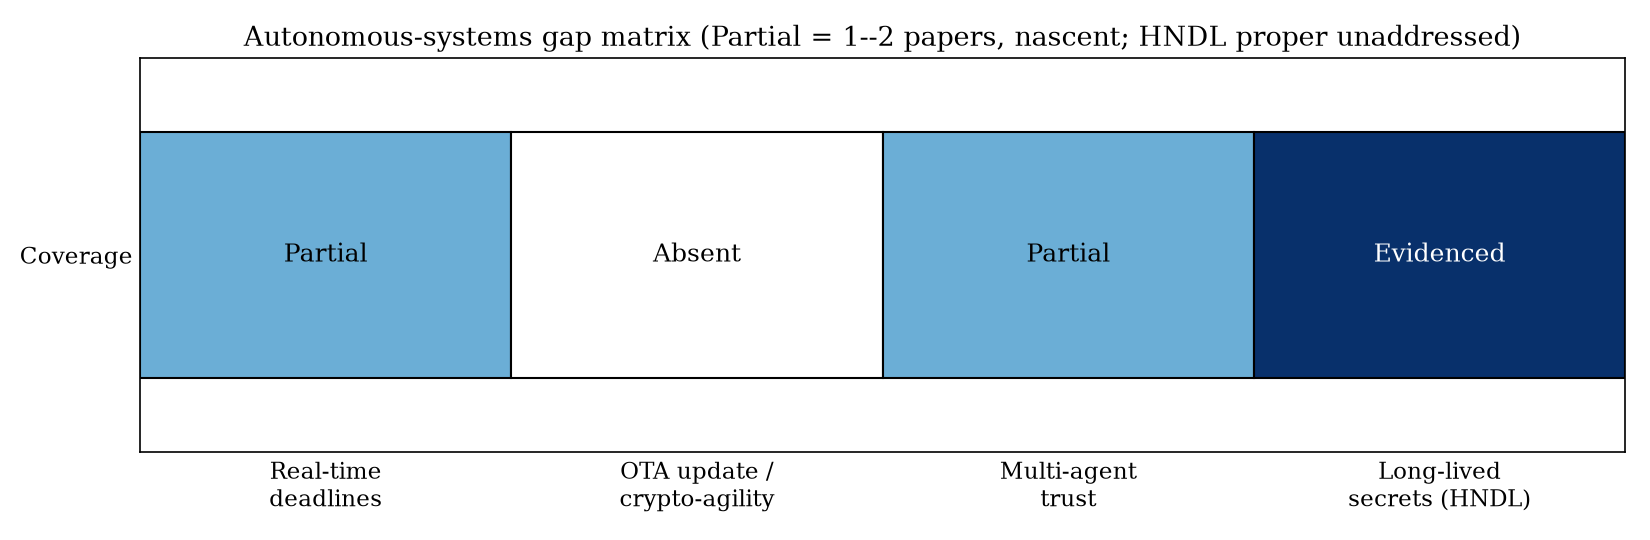
\includegraphics[width=0.95\linewidth]{figures/Fig9_gap_matrix.png}
\caption{Autonomous-systems gap matrix. Real-time deadlines and multi-agent trust are Partial (1--2 papers each: nascent coverage, far from deployment-grade, hence ``essentially unaddressed'' in the abstract); OTA update/crypto-agility is absent; long-lived secrets show short-range key-recovery evidence (BLE far-field SCA) while store-now-decrypt-later against the PQC transition is unaddressed.}
\label{fig:gaps}
\end{figure}

\section{Research Gaps and Future Directions}
\label{sec:gaps}
Cross-referencing the bibliometric analysis of \S\ref{sec:corpus} with the function-level reviews of \S\S\ref{sec:threat}--\ref{sec:cross} yields six structural gaps, summarized in Table~\ref{tab:gaps} and operationalized into the concrete reporting checklist in Table~\ref{tab:checklist}. The ordering is deliberate: the first three rows concern how the field evaluates and shares evidence, the fourth how it reports cost, and the last two where the evidence stops short of deployment needs. None of the six requires a new method family, and all are measurable against the released dataset---a rerun of this review in two years should be able to score each row as narrowed, unchanged, or widened. The checklist is the review's most actionable artifact: the minimum metadata a study must disclose for its claims to be comparable, reproducible, and poolable in future syntheses. Each item corresponds to a practice whose absence the corpus analysis showed to be distorting---undisclosed splits, unnamed datasets, or unquantified compute. Checklist adherence in-corpus is reported only for coded items (descriptive, single-coder): dataset/testbed identity present for 72 testbed-or-collected rows with 32 unclear; adversary model explicit (R1=2) in 39 of 130; split protocol rarely isolated (35 standard/unclear validations); OTA-vs-simulation declared via validation field (47 testbed, 18 sim-only); closed-loop (item 6) at 14 of 121 core (11.6\%) by the rule in \S\ref{sec:cross}; onboard cost present on 16 of 84 defense rows (defense R3 mean 0.19); artifacts released for 4 of 121 core (3.3\%). Items 7--9 and 11 (baselines, seeds, uncertainty, failure analysis) were never coded, so no corpus claim is made about them---they are prospective requirements, as is the checklist as a whole beyond the coded items.
\begin{table}[tbp]
\centering
\footnotesize
\setlength{\tabcolsep}{3pt}
\caption{Structural research gaps and corresponding future directions.}
\label{tab:gaps}
\begin{tabular}{@{}>{\raggedright\arraybackslash}p{3.0cm} >{\raggedright\arraybackslash}p{5.2cm} >{\raggedright\arraybackslash}p{6.4cm}@{}}
\toprule
Gap & Evidence & Direction \\
\midrule
Closed-loop evaluation & Dual-track 7/130 (5.4\%); dual R2 1.14 lowest (margin 0.13 at n=7); broader measure 14/130 & Adversarial-benchmark suites with OTA mandates \\
Reproducibility & 3.3\% verified releases (4/121 core); R4 means 0.00--0.07 & Artifact-evaluated security tracks; dataset DOIs \\
Standards alignment & 9.9\% outside PQC (13.1\% incl. PQC); RFF nearly zero; defense R5 0.07 & Authentication profiles (3GPP/IETF) for learned PHY-auth \\
Onboard cost & DRL/semantic cost-silent; defense R3 0.19 (16/84 rows) & Latency/energy/memory as required reporting \\
Autonomous trust & 1--2 papers per need & Real-time auth, OTA agility, swarm insider models \\
AI$\times$PQC join & Empty in-corpus (non-radio proximity study excluded) & ML-SCA of PQC over the air; migration prioritization \\
\bottomrule
\end{tabular}
\end{table}

\begin{table}[tbp]
\centering
\footnotesize
\setlength{\tabcolsep}{3pt}
\caption{Proposed WIRELESS-AI-RC reporting checklist (12 items).}
\label{tab:checklist}
\begin{tabular}{@{}l >{\raggedright\arraybackslash}p{3.8cm} >{\raggedright\arraybackslash}p{10.0cm}@{}}
\toprule
\# & Item & Must report \\
\midrule
1 & Dataset/testbed identity & Name, version, download or testbed description \\
2 & Device/link population & Radios, channels, distances, day/receiver splits \\
3 & Adversary model & Knowledge, capability, RF/compute budget \\
4 & Split protocol & Within/cross-receiver/day/domain $+$ isolation argument \\
5 & OTA vs simulation & Declaration; sim-only flagged as such \\
6 & Closed-loop evaluation & Attack paper: defenses tested; defense paper: attacks tested \\
7 & Baselines & $\ge$1 classical alongside proposed method, identical data \\
8 & Randomness & Seeds or repeated-run statistics \\
9 & Uncertainty & Error bars, not point estimates alone \\
10 & Onboard cost & Latency/energy/memory on stated platform \\
11 & Failure analysis & $\ge$1 documented failure mode $+$ distribution \\
12 & Artifacts & Code/data DOI or explicit exemption \\
\bottomrule
\end{tabular}
\end{table}
We suggest venues adopt the checklist as a submission requirement and authors attach it to their released datasets: it costs little, and it is what lets the next synthesis do its job.

\section{Conclusion}
\label{sec:conclusion}
Three conclusions stand out, answering the title question for the research literature directly: no---the published literature does not demonstrate wireless security ready for the AI era on current evidence (a statement about literature maturity, not a measurement of deployed systems). First, the method center moved from fingerprint classifiers to adversarial science---attacks are cheap, largely demonstrated on captures/testbeds (threat plurality 16/30 testbed, not norm), and OTA-demonstrated in the strongest cases. Second, the application center stayed in RFFI accuracy, which is not authentication---defenses are rarely adversarially evaluated (broader closed-loop 14/121 core (11.6\%); dual-track detail in \S\ref{sec:cross}). Third, readiness does not follow publication volume: reproducibility, standards, onboard cost, and autonomous-trust evidence trail accuracy claims in volume and maturity---and venue channels differ modestly on rigor: validation rigor runs close across channels (testbed 40\% journals vs 30\% conferences; R2 1.40 vs 1.26, gaps small relative to arm sizes) (\S\ref{sec:sensitivity}). If the last five years were about discovering what learning can extract from radio signals, the next five will be decided by what it can be trusted to protect---under adaptive adversaries, on constrained radios, at fleet scale.

\section*{Declarations}
Funding.\ No specific funding for this work. Conflicts.\ None declared. Author contributions.\ Screener 1 performed 100\% title/abstract screening, full-text eligibility review, charting, and drafting; Verifiers A and B performed corrective checks and revision. Data availability.\ The classified corpus (\texttt{dataset\_papers.csv}), screening log, retrieval records, and analysis scripts accompany this submission as an anonymized supplementary archive; a public repository will be named upon acceptance. Code availability.\ Coding and figure-generation scripts are included in the supplementary archive and rerun from the released dataset; \texttt{check\_consistency.py} gates export. Ethics.\ Not applicable. AI use.\ AI assistance was limited to candidate pooling, prose drafting, and copy-editing; no screening, coding, counting, or verification decision was delegated to AI, and all counts were regenerated programmatically from the released dataset under human control (Screener 1; Verifiers A and B; no blind $\kappa$ claimed). Every record carries a resolvable identifier verified against Crossref, arXiv, ACM, or USENIX; no identifier was fabricated or shared. The authors take full responsibility for the content.

\section*{References (corpus, keyed by corpus ID)}
Corpus IDs (e.g.\ [T30]) are the citation keys used in the text. The full classified dataset maps each ID to its coding.
% Auto-generated from data/found_papers.csv — do not hand-edit.
\begin{enumerate}
\item[D01] Coutaud et al., ``Learning asymmetric encryption using adversarial neural networks,'', Engineering Applications of Artificial Intelligence (Elsevier), 2023. \url{https://www.sciencedirect.com/science/article/abs/pii/S0952197623004049}
\item[D02] Guo Y; Zhang J; Hong Y-WP, ``Practical Physical Layer Authentication for Mobile Scenarios Using a Synthetic Dataset Enhanced Deep Learning Approach,'', IEEE Trans Inf Forensics Secur, 2025. \url{https://doi.org/10.1109/TIFS.2025.3602265}
\item[D03] Wang R; Tang J; Shi Y; Chang SY, ``Deep Learning Based Adaptive Physical Layer Key Distribution,'', IEEE NCIC, 2023. \url{https://doi.org/10.1109/NCIC61838.2023.00046}
\item[D04] Dentremont C; Liu H, ``Deep Learning Dataset Generation for Physical Layer Authentication in Wireless Sensor Networks (WSN),'', IEEE IWCMC, 2024. \url{https://doi.org/10.1109/IWCMC61514.2024.10592476}
\item[D05] Li J; Zhang S; Xing M; Qiao Z; Zhang X, ``Mobile Device Identification Based on Two-dimensional Representation of RF Fingerprint with Deep Learning,'', IEEE ISCC, 2022. \url{https://doi.org/10.1109/ISCC55528.2022.9913038}
\item[D06] Lu Z; Wang T; Liu X; Li N, ``Deep Learning Based Wireless Device Identification Using RF Fingerprint,'', IEEE NNICE, 2023. \url{https://ieeexplore.ieee.org/document/10105692}
\item[D07] Shen G; Zhang J; Marshall A; Woods R, ``Towards Receiver-Agnostic and Collaborative Radio Frequency Fingerprint Identification,'', IEEE Trans Mobile Computing, 2024. \url{https://doi.org/10.1109/tmc.2023.3340039}
\item[D08] Papangelo L; et al., ``Adversarial machine learning for image-based radio frequency fingerprinting: Attacks and defenses,'', IEEE Communications Magazine vol 62(11) pp 108-113, 2024. \url{https://ieeexplore.ieee.org/document/10384628}
\item[D09] Feng C; Sun L, ``Physical Layer Key Generation from Wireless Channels with Non-ideal Channel Reciprocity: A Deep Learning Based Approach,'', IEEE VTC Spring, 2022. \url{https://doi.org/10.1109/VTC2022-Spring54318.2022.9860995}
\item[D10] Chen C; Zhang J; Lu T; Sandell M; Chen L, ``Machine Learning-Based Secret Key Generation for IRS-assisted Multi-antenna Systems,'', IEEE ICC, 2023. \url{https://arxiv.org/abs/2301.08179}
\item[D11] Zhang X; Li G; Zhang J; Hu A; Xiao B, ``Deep Learning-based Physical-Layer Secret Key Generation for FDD Systems (KGNet),'', IEEE Internet of Things Journal, 2021. \url{https://doi.org/10.1109/jiot.2021.3109272}
\item[D12] Jiao L; Sun G; Le J; Zeng K, ``Machine Learning-Assisted Wireless PHY Key Generation with Reconfigurable Intelligent Surfaces,'', ACM WiseML, 2021. \url{https://doi.org/10.1145/3468218.3469042}
\item[D13] Shi Y; Tang J; Wang R; Wen H, ``Physical Layer Key Distribution Technology on Deep Learning,'', IEEE NCIC, 2023. \url{https://doi.org/10.1109/ncic61838.2023.00027}
\item[D14] Liu X; Wang X; Xu Y; Du Z; Xu Y; Han H, ``Lightweight Reinforcement Learning with State Abstraction for Dynamic Spectrum Anti-Jamming Communications,'', IEEE WCNC, 2024. \url{https://doi.org/10.1109/WCNC57260.2024.10571324}
\item[D15] Lv Z; Xiao L; Du Y; Niu G, ``Multi-Agent Reinforcement Learning Based UAV Swarm Communications Against Jamming,'', IEEE Trans Wireless Commun vol 22(12), 2023. \url{https://doi.org/10.1109/twc.2023.3268082}
\item[D16] Shao Z; Yang H; Xiao L; et al., ``Deep Reinforcement Learning-Based Resource Management for UAV-Assisted Mobile Edge Computing Against Jamming,'', IEEE Trans Mobile Computing vol 23(12), 2024. \url{https://doi.org/10.1109/TMC.2024.3432491}
\item[D17] Su G; Dai M; Chen B; Lin X, ``Reinforcement Learning Aided Secure UAV Communications against Roaming Adversaries,'', IEEE ICOIN, 2024. \url{https://doi.org/10.1109/ICOIN59985.2024.10572192}
\item[D18] Zhou; Wang; Ma; Fan; Xiao, ``Physical Layer Authentication for UAV Communications Under Rayleigh and Rician Channels,'', IEEE Trans Wireless Commun vol 24 pp 2722-2733, 2025. \url{https://doi.org/10.1109/TWC.2024.3524210}
\item[D19] Amin H; Kaldari J; Mohamed N; Aman W; Al-Kuwari S, ``Hybrid PLS-ML Authentication Scheme for V2I,'', IEEE ISNCC, 2023. \url{https://doi.org/10.1109/isncc58260.2023.10323824}
\item[D20] Cheng Q; et al., ``Physical Layer Authentication in UAV Communications (spoofing),'', IEEE Transactions on Vehicular Technology, 2025. \url{https://doi.org/10.1109/tvt.2025.3532982}
\item[D21] Song; Guo; Hu; Yang, ``Deep Reinforcement Learning-Based Anti-Jamming Rate Adaptation (UAV ad hoc),'', IEEE Trans Consumer Electronics (Nov), 2025. \url{https://doi.org/10.1109/tce.2025.3627267}
\item[D22] Dong; Wang; Tian; Cheng, ``Deep Reinforcement Learning Based UAV for Securing mmWave Communications,'', IEEE Trans Vehicular Technology (Apr), 2023. \url{https://doi.org/10.1109/tvt.2022.3224959}
\item[D23] Zhang Z; Guo Y; Fang Y; Gong Y, ``Communication and Energy Efficient Wireless Federated Learning with Intrinsic Privacy (PFELS),'', IEEE Trans Dependable Secure Comput, 2023. \url{https://arxiv.org/abs/2304.07460}
\item[D24] Seif M; Tandon R; Li M, ``Wireless Federated Learning with Local Differential Privacy,'', IEEE ISIT 2020 (pp 2604-2609), 2020. \url{https://doi.org/10.1109/ISIT44484.2020.9174426}
\item[D25] Aghdam SR; Amid E; Furdek M; Graell i Amat A, ``Privacy-Preserving Wireless Federated Learning Exploiting Inherent Hardware Impairments,'', IEEE CAMAD Workshops, 2021. \url{https://doi.org/10.1109/camad52502.2021.9617764}
\item[D26] Mao J; et al., ``Providing Differential Privacy for Federated Learning Over Wireless: A Cross-layer Framework,'', IEEE ICC (presented per authors), 2024. \url{https://arxiv.org/abs/2412.04408}
\item[D27] Wu; Chen; Sun; Fang, ``Open Set RF Fingerprint Identification for Wireless Communications,'', IEEE Wireless Commun Lett (Mar), 2025. \url{https://doi.org/10.1109/lwc.2024.3523271}
\item[D28] Xie W; et al., ``A Novel Radio Frequency Fingerprint Identification Scheme for Few-shot Open-set Recognition,'', IEEE Internet of Things Journal vol 12 pp 25691-25706, 2025. \url{https://doi.org/10.1109/jiot.2025.3559183}
\item[D29] Liu; Zhao; Chen, ``A Novel Framework for Few-Shot RF Fingerprint Identification Using Signal Recurrence Plot and Broad Learning,'', IEEE Commun Lett (Sep), 2025. \url{https://doi.org/10.1109/lcomm.2025.3588073}
\item[D30] Cai; Shan; Gao; He, ``Open Set RF Fingerprinting Identification: A Joint Prediction and Siamese Comparison Framework,'', IEEE ICC, 2025. \url{https://doi.org/10.1109/icc52391.2025.11160882}
\item[D31] Ma Z; Fang S; Fan Y, ``Open-Set Radio Frequency Fingerprint Identification Based on Multi-Task Prototype Learning,'', Sensors, 2025. \url{https://doi.org/10.3390/s25175415}
\item[D32] Huang Y; Li R; Chen M; Zhao F; Zhang D; Tu W, ``Securing UAV Communications by Fusing Cross-Layer Fingerprints (SecureLink),'', IEEE Internet of Things Journal, 2025. \url{https://doi.org/10.1109/jiot.2025.3631020}
\item[D33] Tyler JH; Fadul MKM; Reising DR, ``Random Adversarial Data Obfuscation Model (RANDOM) Adversarial Neural Cryptography,'', venue unconfirmed (arXiv 2411.10287), 2024. \url{https://arxiv.org/abs/2411.10287}
\item[D34] Abdalla AS; Behfarnia A; Marojevic V, ``Aerial Base Station Positioning and Power Control for Securing Communications: A Deep Q-Network Approach,'', IEEE WCNC, 2022. \url{https://doi.org/10.1109/wcnc51071.2022.9771893}
\item[D35] Hoseini SA; Bouhafs F; Aboutorab N, ``Cooperative Jamming for Physical Layer Security Enhancement Using Deep Reinforcement Learning,'', IEEE GLOBECOM Workshops, 2023. \url{https://doi.org/10.1109/gcwkshps58843.2023.10465104}
\item[D36] Sahay R; Brinton CG; Love DJ, ``A Deep Ensemble-based Wireless Receiver Architecture for Mitigating Adversarial Attacks in Automatic Modulation Classification,'', IEEE Trans Cogn Commun Networking (Mar 2022), 2022. \url{https://doi.org/10.1109/tccn.2021.3114154}
\item[D37] Meng; Qi; Zheng; Cai; Zhou; Jiang, ``Adversarial Attack and Reliable Defense Based on Frequency Domain Feature Enhancement for Automatic Modulation Classification,'', IEEE Trans Inf Forensics Secur vol 20 pp 3731-3744, 2025. \url{https://doi.org/10.1109/TIFS.2025.3553806}
\item[D38] Gao N; Han Y; Li N; Jin S; Matthaiou M, ``When Physical Layer Key Generation Meets RIS: Opportunities Challenges and Road Ahead,'', IEEE Wireless Communications, 2024. \url{https://doi.org/10.1109/mwc.013.2200538}
\item[D39] Alwazani H; Chaaban A, ``Disruptive RIS for Enhancing Key Generation and Secret Transmission in Low-Entropy Environments,'', venue unconfirmed (arXiv 2409.15303), 2024. \url{https://arxiv.org/abs/2409.15303}
\item[D40] Guo J; Gao N; Zuo Y; Xu H; Jin S; Wong KK, ``A Fluid Antenna Enabled Physical Layer Key Generation for Next-G Wireless Networks,'', IEEE WCSP, 2025. \url{https://doi.org/10.1109/wcsp68525.2025.1010537}
\item[D41] Zhang X; Li G; Zhang J; et al., ``Enabling Deep Learning-based Physical-layer Secret Key Generation for FDD-OFDM Systems in Multi-Environments,'', IEEE Trans Vehicular Technology (accepted per arXiv), 2024. \url{https://arxiv.org/abs/2211.03065}
\item[D42] Shahiri V; Li G; Behroozi H, ``RIS-Assisted Physical Layer Group Key Generation,'', venue unconfirmed (arXiv 2507.00714; under review), 2025. \url{https://arxiv.org/abs/2507.00714}
\item[D43] Chen Z, ``Secure-IRS: Defending Against Adversarial Physical-Layer Sensing,'', IEEE ICNC 2025 (pp 436-440), 2025. \url{https://doi.org/10.1109/ICNC64010.2025.10993984}
\item[D44] Chen J; Wong W-K; Hamdaoui B, ``Unsupervised Contrastive Learning for Robust RF Device Fingerprinting Under Time-Domain Shift,'', IEEE ICC, 2024. \url{https://arxiv.org/abs/2403.04036}
\item[D45] Razak FA; Yilmaz Y, ``Dynamic and Open-Set RF Fingerprinting and Localization in Crowded Indoor Environments through Contrastive CSI Learning,'', venue unconfirmed (arXiv 2605.15593), 2026. \url{https://arxiv.org/abs/2605.15593}
\item[D46] Zeng S; Shen Y; Zhang Y; Shen Y; Tan Z; Song HH, ``HoRFFI: High-Openness RF Fingerprint Identification with Similarity-Enhanced Variational Information Bottleneck,'', venue unconfirmed (arXiv 2608.04881; INFOCOM-2026 submission label inconsistent with Aug-2026 posting), 2026. \url{https://arxiv.org/abs/2608.04881}
\item[D47] Parpart GG; et al., ``Transformer Masked Autoencoders for RF Device Fingerprinting,'', IEEE MILCOM, 2024. \url{https://doi.org/10.1109/MILCOM61039.2024.10773654}
\item[D48] Mahajan A; Burleson W, ``Watermarking and Anomaly Detection in Machine Learning Models for LoRa RF Fingerprinting,'', IEEE ICASSP (per arXiv comment), 2025. \url{https://arxiv.org/abs/2509.15170}
\item[D49] Johnson B; Albousayri H; Hamdaoui B, ``Domain-Adaptive Device Fingerprints for Network Access Authentication,'', IEEE Network, 2025. \url{https://doi.org/10.1109/mnet.2025.3587300}
\item[D50] Puppo L; Wong W-K; Hamdaoui B, ``HiNoVa: A Novel Open-set Detection Method for Automating RF Device Authentication,'', IEEE ISCC, 2023. \url{https://doi.org/10.1109/iscc58397.2023.10217841}
\item[D52] Amiriara H; et al., ``A Physical Layer Security Framework for IRS-Assisted Integrated Sensing and Semantic Communication Systems,'', IEEE Trans Cogn Commun Networking vol 11 pp 2955-2969, 2025. \url{https://doi.org/10.1109/TCCN.2025.3589577}
\item[D53] Li Y; Shi Z; Hu H; Fu Y; Wang H; Lei H, ``Secure Semantic Communications: From Perspective of Physical Layer Security,'', IEEE Communications Letters, 2024. \url{https://doi.org/10.1109/lcomm.2024.3452715}
\item[D54] Huang S; Zhou Y; Wang T; Shi Y, ``Byzantine-Resilient Federated Machine Learning via Over-the-Air Computation,'', IEEE ICC Workshops, 2021. \url{https://doi.org/10.1109/iccworkshops50388.2021.9473694}
\item[D55] Hanna S; Karunaratne S; Cabric D, ``Open Set Wireless Transmitter Authorization: Deep Learning Approaches and Dataset Considerations,'', IEEE Trans Cogn Commun Networking vol 7 pp 59-72, 2021. \url{https://doi.org/10.1109/tccn.2020.3043332}
\item[D56] Shen G; Zhang J; Marshall A; et al., ``Radio frequency fingerprint identification for LoRa using deep learning,'', IEEE J Sel Areas Commun vol 39 pp 2604-2616, 2021. \url{https://doi.org/10.1109/jsac.2021.3087250}
\item[D57] Rajendran S; Sun Z, ``RF impairment model-based IoT physical-layer identification for enhanced domain generalization,'', IEEE Trans Inf Forensics Secur vol 17 pp 1285-1299, 2022. \url{https://doi.org/10.1109/tifs.2022.3158553}
\item[D58] Jagannath A; Jagannath J, ``Embedding-assisted attentional deep learning for real-world RF fingerprinting of Bluetooth,'', IEEE Trans Cogn Commun Networking vol 9 pp 940-949, 2023. \url{https://doi.org/10.1109/tccn.2023.3269764}
\item[D59] Jiang Q; Sha J, ``Radio frequency fingerprint identification in low SNR scenarios for automatic identification system,'', IEEE Trans Wireless Commun vol 23 pp 2070-2081, 2024. \url{https://doi.org/10.1109/twc.2023.3294988}
\item[D60] Kong; Chen, ``DeepCRF: Deep learning-enhanced CSI-based RF fingerprinting for channel-resilient WiFi device identification,'', IEEE Trans Inf Forensics Secur, 2025. \url{https://doi.org/10.1109/tifs.2024.3515796}
\item[D61] Yang; Feng; Wang; Wu, ``OpenRFI: Open-Set Radio Frequency Fingerprint Identification via Test-Time Fine-Tuning,'', IEEE Trans Mobile Computing (Nov), 2025. \url{https://doi.org/10.1109/tmc.2025.3582980}
\item[D62] Hu Y; Du Y; et al., ``Few-shot cross-receiver radio frequency fingerprinting identification based on feature separation,'', IET Communications vol 18, 2024. \url{https://doi.org/10.1049/cmu2.12841}
\item[D63] Wang W; Liao H; Gan L, ``Open-Set RF Fingerprinting via Improved Prototype Learning,'', venue unconfirmed (arXiv 2306.13895), 2023. \url{https://arxiv.org/abs/2306.13895}
\item[D64] Zhao T; et al., ``Cross-domain, scalable, and interpretable RF device fingerprinting,'', IEEE INFOCOM (pp 2099-2108), 2024. \url{https://doi.org/10.1109/infocom52122.2024.10621423}
\item[D65] Zhao T; et al., ``Few-shot learning and data augmentation for cross-domain UAV fingerprinting,'', ACM MobiCom (pp 2389-2394), 2024. \url{https://doi.org/10.1145/3636534.3698248}
\item[D66] Yin P; et al., ``Multi-Channel CNN-Based Open-Set RF Fingerprint Identification for LTE Devices,'', IEEE Trans Cogn Commun Networking, 2024. \url{https://ieeexplore.ieee.org/document/10505882}
\item[D67] Pei S; Huang S; Liu H; et al., ``Proactive Radio Frequency Fingerprinting-Based Authentication Leverage IQ Perturbation,'', IEEE TrustCom (pp 556-565), 2025. \url{https://doi.org/10.1109/Trustcom66490.2025.00068}
\item[D68] Li Y-T; Liu Y; Su J; Yang X, ``SV-NPR: an Open-Set RF Fingerprint Identification Framework Based on Siamese Network,'', IEEE ISCC, 2025. \url{https://doi.org/10.1109/ISCC65549.2025.11326374}
\item[D69] Yang; Bao; Zhang; Wang, ``A Hybrid Model With Bayesian Nonparametric Inference for RF Fingerprint Identification,'', IEEE Trans Mobile Computing (Feb), 2026. \url{https://doi.org/10.1109/tmc.2025.3611135}
\item[D70] Elmaghbub A; Hamdaoui B, ``No Blind Spots: On the Resiliency of Device Fingerprints to Hardware Warm-Up Through Sequential Transfer Learning,'', ACM WiSec, 2024. \url{https://doi.org/10.1145/3643833.3656138}
\item[D71] Oligeri G; Sciancalepore S; Raponi S; Di Pietro R, ``PAST-AI: Physical-Layer Authentication of Satellite Transmitters via Deep Learning,'', IEEE Trans Inf Forensics Secur, 2022. \url{https://doi.org/10.1109/tifs.2022.3219287}
\item[D72] Elmaghbub A; Hamdaoui B, ``Distinguishable IQ Feature Representation for Domain-Adaptation Learning of WiFi Device Fingerprints,'', IEEE Trans Mach Learn Commun Netw, 2024. \url{https://doi.org/10.1109/tmlcn.2024.3446743}
\item[D73] Ahmed A; Quoitin B; Fontaine J; Shahid A, ``On the Generalization of Deep Learning Based Radio Frequency Fingerprint Identification System in a Multi-Distance Scenario,'', IEEE PIMRC, 2025. \url{https://doi.org/10.1109/pimrc62392.2025.11275484}
\item[D74] Sanchez Viloria JA; Sklivanitis G; Pados D; Bentley ES, ``Channel-Informed Neural Network for Physical Layer Key Generation,'', venue unconfirmed (arXiv 2609.16341), 2026. \url{https://arxiv.org/abs/2609.16341}
\item[D75] He J; Wang Y; He F; Huang S, ``Deep Learning based Cross-Receiver Radio Frequency Fingerprint Identification Under Varying Channels,'', venue unconfirmed (arXiv 2603.08402), 2026. \url{https://arxiv.org/abs/2603.08402}
\item[D76] Liu C; Meng R; Liu Y; Xu X, ``IPRU: Input-Perturbation-based Radio Frequency Fingerprinting Unlearning for LAWNs,'', venue unconfirmed (arXiv 2604.24022), 2026. \url{https://arxiv.org/abs/2604.24022}
\item[D77] Yin Z; Li J; Wang Z; Qian Y, ``UAV Communication Against Intelligent Jamming: A Stackelberg Game Approach With Federated Reinforcement Learning,'', IEEE Trans Green Commun Netw, 2024. \url{https://doi.org/10.1109/tgcn.2024.3373886}
\item[D78] Tiantian Zhang; Pinyi Ren; Zhanyi Ren, ``Deep Radio Fingerprint ResNet for Reliable Lightweight Device Identification,'', IEEE Vehicular Technology Conference, 2021. \url{https://doi.org/10.1109/vtc2021-fall52928.2021.9625375}
\item[D79] Jing Ma; Pinyi Ren; Tiantian Zhang; Zhanyi Ren, ``Deep Radio Frequency Fingerprinting Based on Wavelet Scattering Network,'', IEEE Wireless Communications and Networking Conference, 2023. \url{https://doi.org/10.1109/wcnc55385.2023.10119009}
\item[D80] Aishwarya Jawne; Georgios Sklavanitis; Dimitris A. Pados; Elizabeth Serena Bentley, ``AI-Assisted RF Fingerprinting for Identification of User Devices in 5G and FutureG,'', FutureG Symposium, 2025. \url{https://doi.org/10.14722/futureg.2025.23009}
\item[D81] Shenhua Wang; Hongliang Jiang; Xiaofang Fang; Yulong Ying, ``Radio Frequency Fingerprint Identification Based on Deep Complex Residual Network,'', IEEE Access, 2020. \url{https://doi.org/10.1109/access.2020.3037206}
\item[D82] Kang Wei; Jun Li; Chuan Ma; Ming Ding, ``Low-Latency Federated Learning over Wireless Channels with Differential Privacy,'', arXiv, 2021. \url{https://doi.org/10.48550/arxiv.2106.13039}
\item[D83] Anis Elgabli; Jihong Park; Chaouki Ben Issaid; Mehdi Bennis, ``Harnessing Wireless Channels for Scalable and Privacy-Preserving Federated Learning,'', IEEE Transactions on Communications, 2021. \url{https://doi.org/10.1109/tcomm.2021.3078783}
\item[D84] Anthony Ayli; Khalil Harris; Jihad Fahs; Mohamad Assaad, ``Privacy-Enhanced Zero-Order Federated Learning via xMK-CKKS over Wireless Channels,'', arXiv, 2026. \url{https://doi.org/10.48550/arxiv.2605.30123}
\item[D85] Shuzhen Chen; Dongxiao Yu; Yifei Zou; Jiguo Yu, ``Decentralized Wireless Federated Learning with Differential Privacy,'', arXiv, 2021. \url{https://doi.org/10.48550/arxiv.2109.09142}
\item[D86] Mohamed Seif; Wei-Ting Chang; Ravi Tandon, ``Privacy Amplification for Federated Learning via User Sampling and Wireless Aggregation,'', IEEE International Symposium on Information Theory (ISIT), 2021. \url{https://doi.org/10.1109/isit45174.2021.9518031}
\item[D87] Nima Tavangaran; Mingzhe Chen; Zhaohui Yang; Jose Mairton B. da Silva, ``On differential privacy for federated learning in wireless systems with multiple base stations,'', IET Communications, 2024. \url{https://doi.org/10.1049/cmu2.12722}
\item[D88] Helin Yang; Jun Zhao; Zehui Xiong; Kwok-Yan Lam, ``Privacy-Preserving Federated Learning for UAV-Enabled Networks: Learning-Based Joint Scheduling and Resource Management,'', IEEE Journal on Selected Areas in Communications, 2021. \url{https://doi.org/10.1109/jsac.2021.3088655}
\item[P01] Lopez J; Cadena V; Rahman MS, ``Evaluating Post-Quantum Cryptographic Algorithms on Resource-Constrained Devices,'', IEEE QCE, 2025. \url{https://www.computer.org/csdl/proceedings-article/qce/2025/573602a655/2c5MluHf5tK}
\item[P03] Abdulrahman A; Hwang V; Kannwischer MJ; Sprenkels A, ``Faster Kyber and Dilithium on the Cortex-M4,'', ACNS (LNCS), 2022. \url{https://doi.org/10.1007/978-3-031-09234-3_42}
\item[P04] Kim Y; Yoon S; Seo SC, ``Vectorized Implementation of Kyber and Dilithium on 32-bit ARM Cortex-A,'', IEEE Access, 2024. \url{https://doi.org/10.1109/access.2024.3435451}
\item[P05] Greconici DOC; Kannwischer MJ; Sprenkels A, ``Compact Dilithium Implementations on Cortex-M3 and Cortex-M4,'', IACR TCHES, 2021. \url{https://doi.org/10.46586/tches.v2021.i1.1-24}
\item[P06] Nguyen; Dam; Duong; et al., ``Efficient Hardware Implementation of the Lightweight CRYSTALS-Kyber,'', IEEE Trans Circuits and Systems I (Feb), 2025. \url{https://doi.org/10.1109/tcsi.2024.3443238}
\item[P08] Gonzalez de la Torre MA; Morales Sandoval IA; Freitas de Abreu GT, ``Post-Quantum Wireless-based Key Encapsulation Mechanism via CRYSTALS-Kyber for Resource-Constrained Devices,'', IEEE Access, 2025. \url{https://doi.org/10.1109/access.2025.3560023}
\item[P09] Kudaloor A; Aijaz A, ``Toward Quantum-Safe 6G: Experimental Evaluation of Post-Quantum Cryptography,'', IEEE Communications Standards Magazine (accepted), 2026. \url{https://arxiv.org/abs/2605.06881}
\item[P10] Blanco-Romero J; Garcia-Nino YM; Almenares Mendoza F; Diaz-Sanchez D, ``Post-Quantum Entropy as a Service for Embedded Systems,'', Lecture Notes in Networks and Systems (book chapter), 2025. \url{https://doi.org/10.1007/978-3-032-16995-2_30}
\item[P11] Nasiraee H, ``LAKE: Lattice-Code Accelerated Kyber Encapsulation,'', Int Conf Combinatorics Cryptography Comput Sci (via eprint 2025/2293), 2025. \url{https://eprint.iacr.org/2025/2293}
\item[T01] Wang R; Wang H; Dubrova E, ``Far Field EM Side-Channel Attack on AES Using Deep Learning,'', 4th ACM Workshop on Attacks and Solutions in Hardware Security (ASHES@CCS), 2020. \url{https://doi.org/10.1145/3411504.3421214}
\item[T03] Ma J; Zhang J; Shen G; Marshall A; Chang C-H, ``Adversarial Attacks Against Deep Learning-Based Radio Frequency Fingerprint Identification,'', IEEE Transactions on Mobile Computing vol 25 pp 7831-7844, 2026. \url{https://doi.org/10.1109/TMC.2025.3646257}
\item[T04] Liu B; Zhang H; Wan Y; Zhou F; Wu Q; Ng D, ``Robust Adversarial Attacks on Deep Learning-Based RF Fingerprint Identification,'', IEEE Wireless Communications Letters vol 12(6), 2023. \url{https://doi.org/10.1109/LWC.2023.3259432}
\item[T05] Sagduyu YE; Erpek T, ``Adversarial Attack and Defense for LoRa Device Identification and Authentication via Deep Learning,'', IEEE MILCOM 2023 (preliminary); full version 2024, 2023. \url{https://arxiv.org/abs/2412.21164}
\item[T06] Lu Z; Tu M; Xie X; Xu W, ``Erasing Radio Frequency Fingerprinting via Active Adversarial Perturbation,'', IEEE Trans Network Science and Engineering 2025, 2025. \url{https://doi.org/10.1109/TNSE.2025.3568824}
\item[T08] Ji Y; Dubrova E; Wang R, ``Is Your Bluetooth Chip Leaking Secrets via RF Signals?,'', IEEE ISMVL, 2025. \url{https://doi.org/10.1109/ismvl64713.2025.00035}
\item[T09] Shi Y; Davaslioglu K; Sagduyu YE, ``Generative Adversarial Network in the Air: Deep Adversarial Learning for Wireless Signal Spoofing,'', IEEE Trans Cogn Commun Netw, 2021. \url{https://doi.org/10.1109/tccn.2020.3010330}
\item[T11] Huang; Al-Hourani, ``Physical Layer Spoof Detection and Authentication for IoT,'', IEEE Trans ML in Commun Networking, 2024. \url{https://doi.org/10.1109/tmlcn.2024.3417806}
\item[T12] Zhao T; Tang Z; Zhang T; et al., ``Stealthy Backdoor Attack on RF Signal Classification,'', IEEE ICCCN, 2023. \url{https://doi.org/10.1109/ICCCN58024.2023.10230152}
\item[T14] Shi Y; Sagduyu YE, ``Membership Inference Attack and Defense for Wireless Signal Classifiers with Deep Learning,'', IEEE Trans Mobile Computing, 2023. \url{https://doi.org/10.1109/tmc.2022.3148690}
\item[T15] Karunaratne et al., ``Open Set RF Fingerprinting using Generative Outlier Augmentation,'', IEEE GLOBECOM 2021, 2021. \url{https://arxiv.org/abs/2108.13099}
\item[T16] Zhao T; Wang X; Zhang J; Mao S, ``Explanation-Guided Backdoor Attacks on Model-Agnostic RF Fingerprinting,'', IEEE INFOCOM Workshops, 2024. \url{https://doi.org/10.1109/INFOCOM52122.2024.10621289}
\item[T17] Zhang; Krunz; Ditzler, ``Stealthy Adversarial Attacks on Machine Learning-Based Classifiers of Wireless Signals,'', IEEE Trans ML in Commun Networking, 2024. \url{https://doi.org/10.1109/tmlcn.2024.3366161}
\item[T18] Karunaratne S; Krijestorac E; Cabric D, ``Penetrating RF Fingerprinting-based Authentication with a Generative Adversarial Attack,'', IEEE ICC 2021, 2021. \url{https://doi.org/10.1109/ICC42927.2021.9500893}
\item[T19] Engelberg A; Wool A, ``Classification of Encrypted IoT Traffic Despite Padding and Shaping,'', ACM WPES, 2022. \url{https://doi.org/10.1145/3559613.3563191}
\item[T20] Morales; Bienek-Parrish; Jenkins; Slavin, ``Protocol-agnostic IoT Device Classification on Encrypted Traffic,'', ACM CPS-IoT Week (pp 19-24), 2023. \url{https://doi.org/10.1145/3576914.3587487}
\item[T21] Nakhla; Song; Vandenberghe; Islam, ``Analysis of encrypted wireless traffic for identification of IoT devices,'', IEEE World AI IoT Congress (May), 2025. \url{https://doi.org/10.1109/aiiot65859.2025.11105346}
\item[T22] Haydar J; Kanaan L; Mokdad A; Beydoun A, ``Network Traffic Fingerprinting for IoT Device Identification Using Machine Learning,'', IEEE NTMS 2025 (Paris), 2025. \url{https://doi.org/10.1109/NTMS65597.2025.11076619}
\item[T23] Eleftherakis S; Giustiniano D; Kourtellis N, ``SoK: Evaluating 5G Protocols Against Legacy and Emerging Privacy and Security Attacks,'', ACM WiSec, 2025. \url{https://doi.org/10.1145/3734477.3734716}
\item[T25] Xie H; Tan J; Zhang X; et al., ``Low-Interception Waveform: To Prevent the Recognition of Spectrum Waveform Modulation via Adversarial Examples,'', URSI GASS 2021, 2021. \url{https://doi.org/10.23919/URSIGASS51995.2021.9560360}
\item[T27] Shuvo MNH; Hossain M; Mallik A; Twigg J; Dagefu F, ``FLARE: A Wireless Side-Channel Fingerprinting Attack on Federated Learning,'', IEEE INFOCOM, 2026. \url{https://doi.org/10.1109/infocom59046.2026.11571658}
\item[T28] Huang Q; Wang X; Guo W; Gu G; Hu H, ``Semantics Over Syntax: Uncovering Pre-Authentication 5G Baseband Vulnerabilities,'', 35th USENIX Security Symposium 2026 (pp 457-476), 2026. \url{https://www.usenix.org/conference/usenixsecurity26/presentation/huang-qiqing}
\item[T30] Chang J-W; Sun K; et al., ``Magmaw: Modality-Agnostic Adversarial Attacks on Machine Learning-Based Wireless Communication Systems,'', NDSS, 2025. \url{https://doi.org/10.14722/ndss.2025.23336}
\item[T31] Shah et al., ``System-level Analysis of Adversarial Attacks and Defenses on Intelligence in O-RAN based Cellular Networks,'', ACM WiSec, 2024. \url{https://arxiv.org/abs/2402.06846}
\item[T36] Sabo SM; et al., ``Chained Attacks on Drone-Based Federated Learning: From Network Disruption to Device Impersonation,'', venue unconfirmed (arXiv 2607.20280), 2026. \url{https://arxiv.org/abs/2607.20280}
\item[T38] Bao Z; Lin Y; Zhang S; Li Z; Mao S, ``Threat of adversarial attacks on DL-based IoT device identification,'', IEEE Internet of Things Journal vol 9 pp 9012-9024, 2022. \url{https://doi.org/10.1109/jiot.2021.3120197}
\item[T39] Restuccia F; et al., ``Generalized wireless adversarial deep learning,'', ACM WiseML (2nd Workshop Wireless Secur Mach Learn), 2020. \url{https://doi.org/10.1145/3395352.3402625}
\item[T40] Cao X; Adhikari B; Zhao S; Wu J, ``An Adversarial-Driven Experimental Study on Deep Learning for RF Fingerprinting,'', IEEE MILCOM, 2025. \url{https://doi.org/10.1109/milcom64451.2025.11309917}
\item[T41] Yao Z; Gui G, ``Backdoor Attack on Self-Supervised Learning-Based RFF Identification Using Spectrum Enhanced Insensitive Perturbation Trigger,'', IEEE Trans Inf Forensics Secur, 2025. \url{https://doi.org/10.1109/tifs.2025.3577013}
\item[T42] Xiao F; Huang Y; Zuo Y; Kuang W, ``Over-The-Air Adversarial Attacks on Deep Learning Wi-Fi Fingerprinting (FooLoc),'', venue unconfirmed (arXiv 2301.03760), 2023. \url{https://arxiv.org/abs/2301.03760}
\item[T43] Huang Y; Liu W; Wang H-M, ``Hidden Backdoor Attack: A New Threat to Learning-Aided Physical Layer Authentication,'', IEEE Ucom, 2023. \url{https://doi.org/10.1109/ucom59132.2023.10257584}
\item[T44] Ke D; Wang X; Huang Z, ``Frequency-Selective Adversarial Attack Against Deep Learning-Based Wireless Signal Classifiers,'', IEEE Trans Inf Forensics Secur, 2024. \url{https://doi.org/10.1109/tifs.2024.3352423}
\item[T46] Li C; Zhang X, ``Security Analysis of IoT Traffic Classification Systems Under Adversarial Machine Learning Attacks,'', J Cyber Secur Mobility, 2026. \url{https://doi.org/10.13052/jcsm2245-1439.1547}
\item[T47] Yi Shi; Yalin E. Sagduyu, ``Jamming Attacks on Federated Learning in Wireless Networks,'', arXiv, 2022. \url{https://doi.org/10.48550/arxiv.2201.05172}
\end{enumerate}


\subsection*{Background surveys (not counted in N)}
\begin{itemize}
\item[BG2] Hoang T.~M. et al., ``Physical Layer Authentication and Security Design in the Machine Learning Era,'' IEEE Communications Surveys \& Tutorials vol.~26(3), 2024. \url{https://ieeexplore.ieee.org/document/10428002}
\item[BG3] Jagannath A., Jagannath J., et al., ``A Comprehensive Survey on Radio Frequency (RF) Fingerprinting,'' Computer Networks (Elsevier), 2022. \url{https://arxiv.org/abs/2201.00680}
\item[BG7] Adesina D., Hsieh C.-C., Sagduyu Y.~E., Qian L., ``Adversarial Machine Learning in Wireless Communications Using RF Data: A Review,'' IEEE Communications Surveys \& Tutorials vol.~25, pp.~77--100, 2023. \url{https://doi.org/10.1109/COMST.2022.3205184}
\end{itemize}
The review protocol (\texttt{protocol.md}) and a PRISMA-ScR checklist mapping each item to its manuscript section accompany the supplementary archive.

\end{document}
